\section{Introduction}

\begin{figure}[t]
	\centering
	\begin{subfigure}[b]{0.23\textwidth}
		\centering
		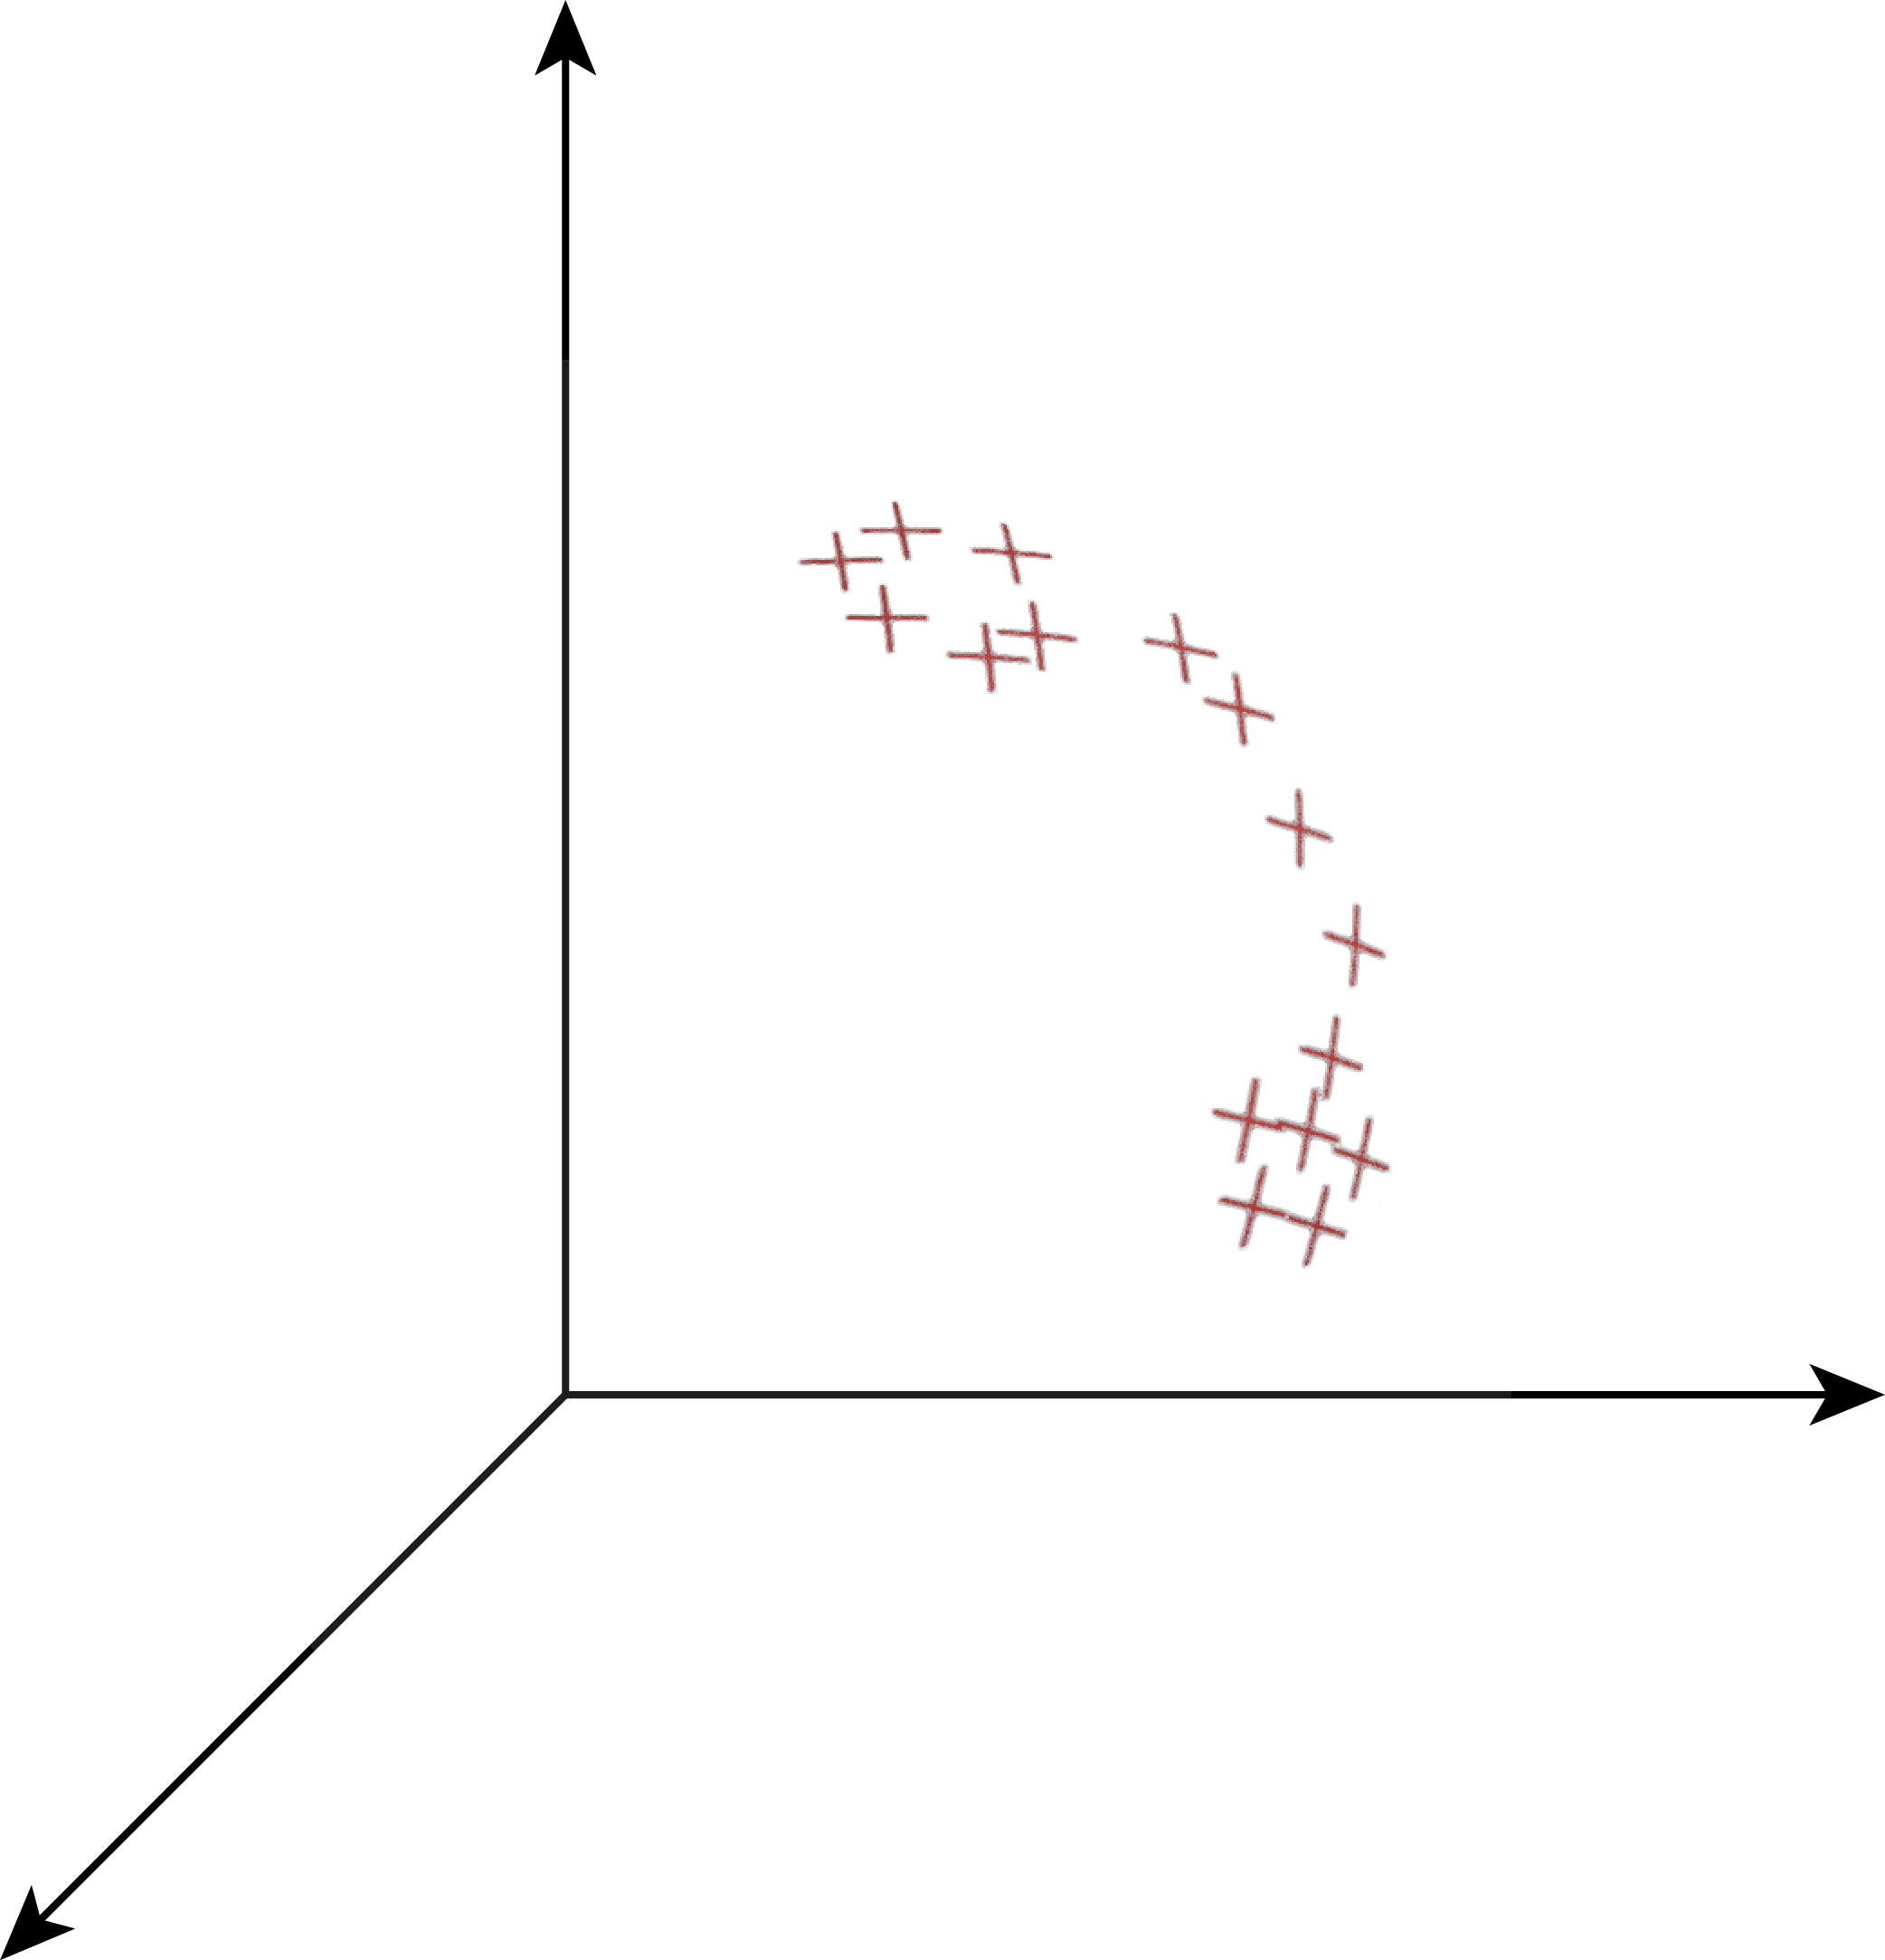
\includegraphics[width=\linewidth]{images/constraind_diffusion_rejection/intro_figure_euclidean@600x-100.jpg}
		\caption{\(\R^3\)}
		\label{fig:intro_figure_euclidean}
	\end{subfigure}
	\hfill
	\begin{subfigure}[b]{0.23\textwidth}
		\centering
		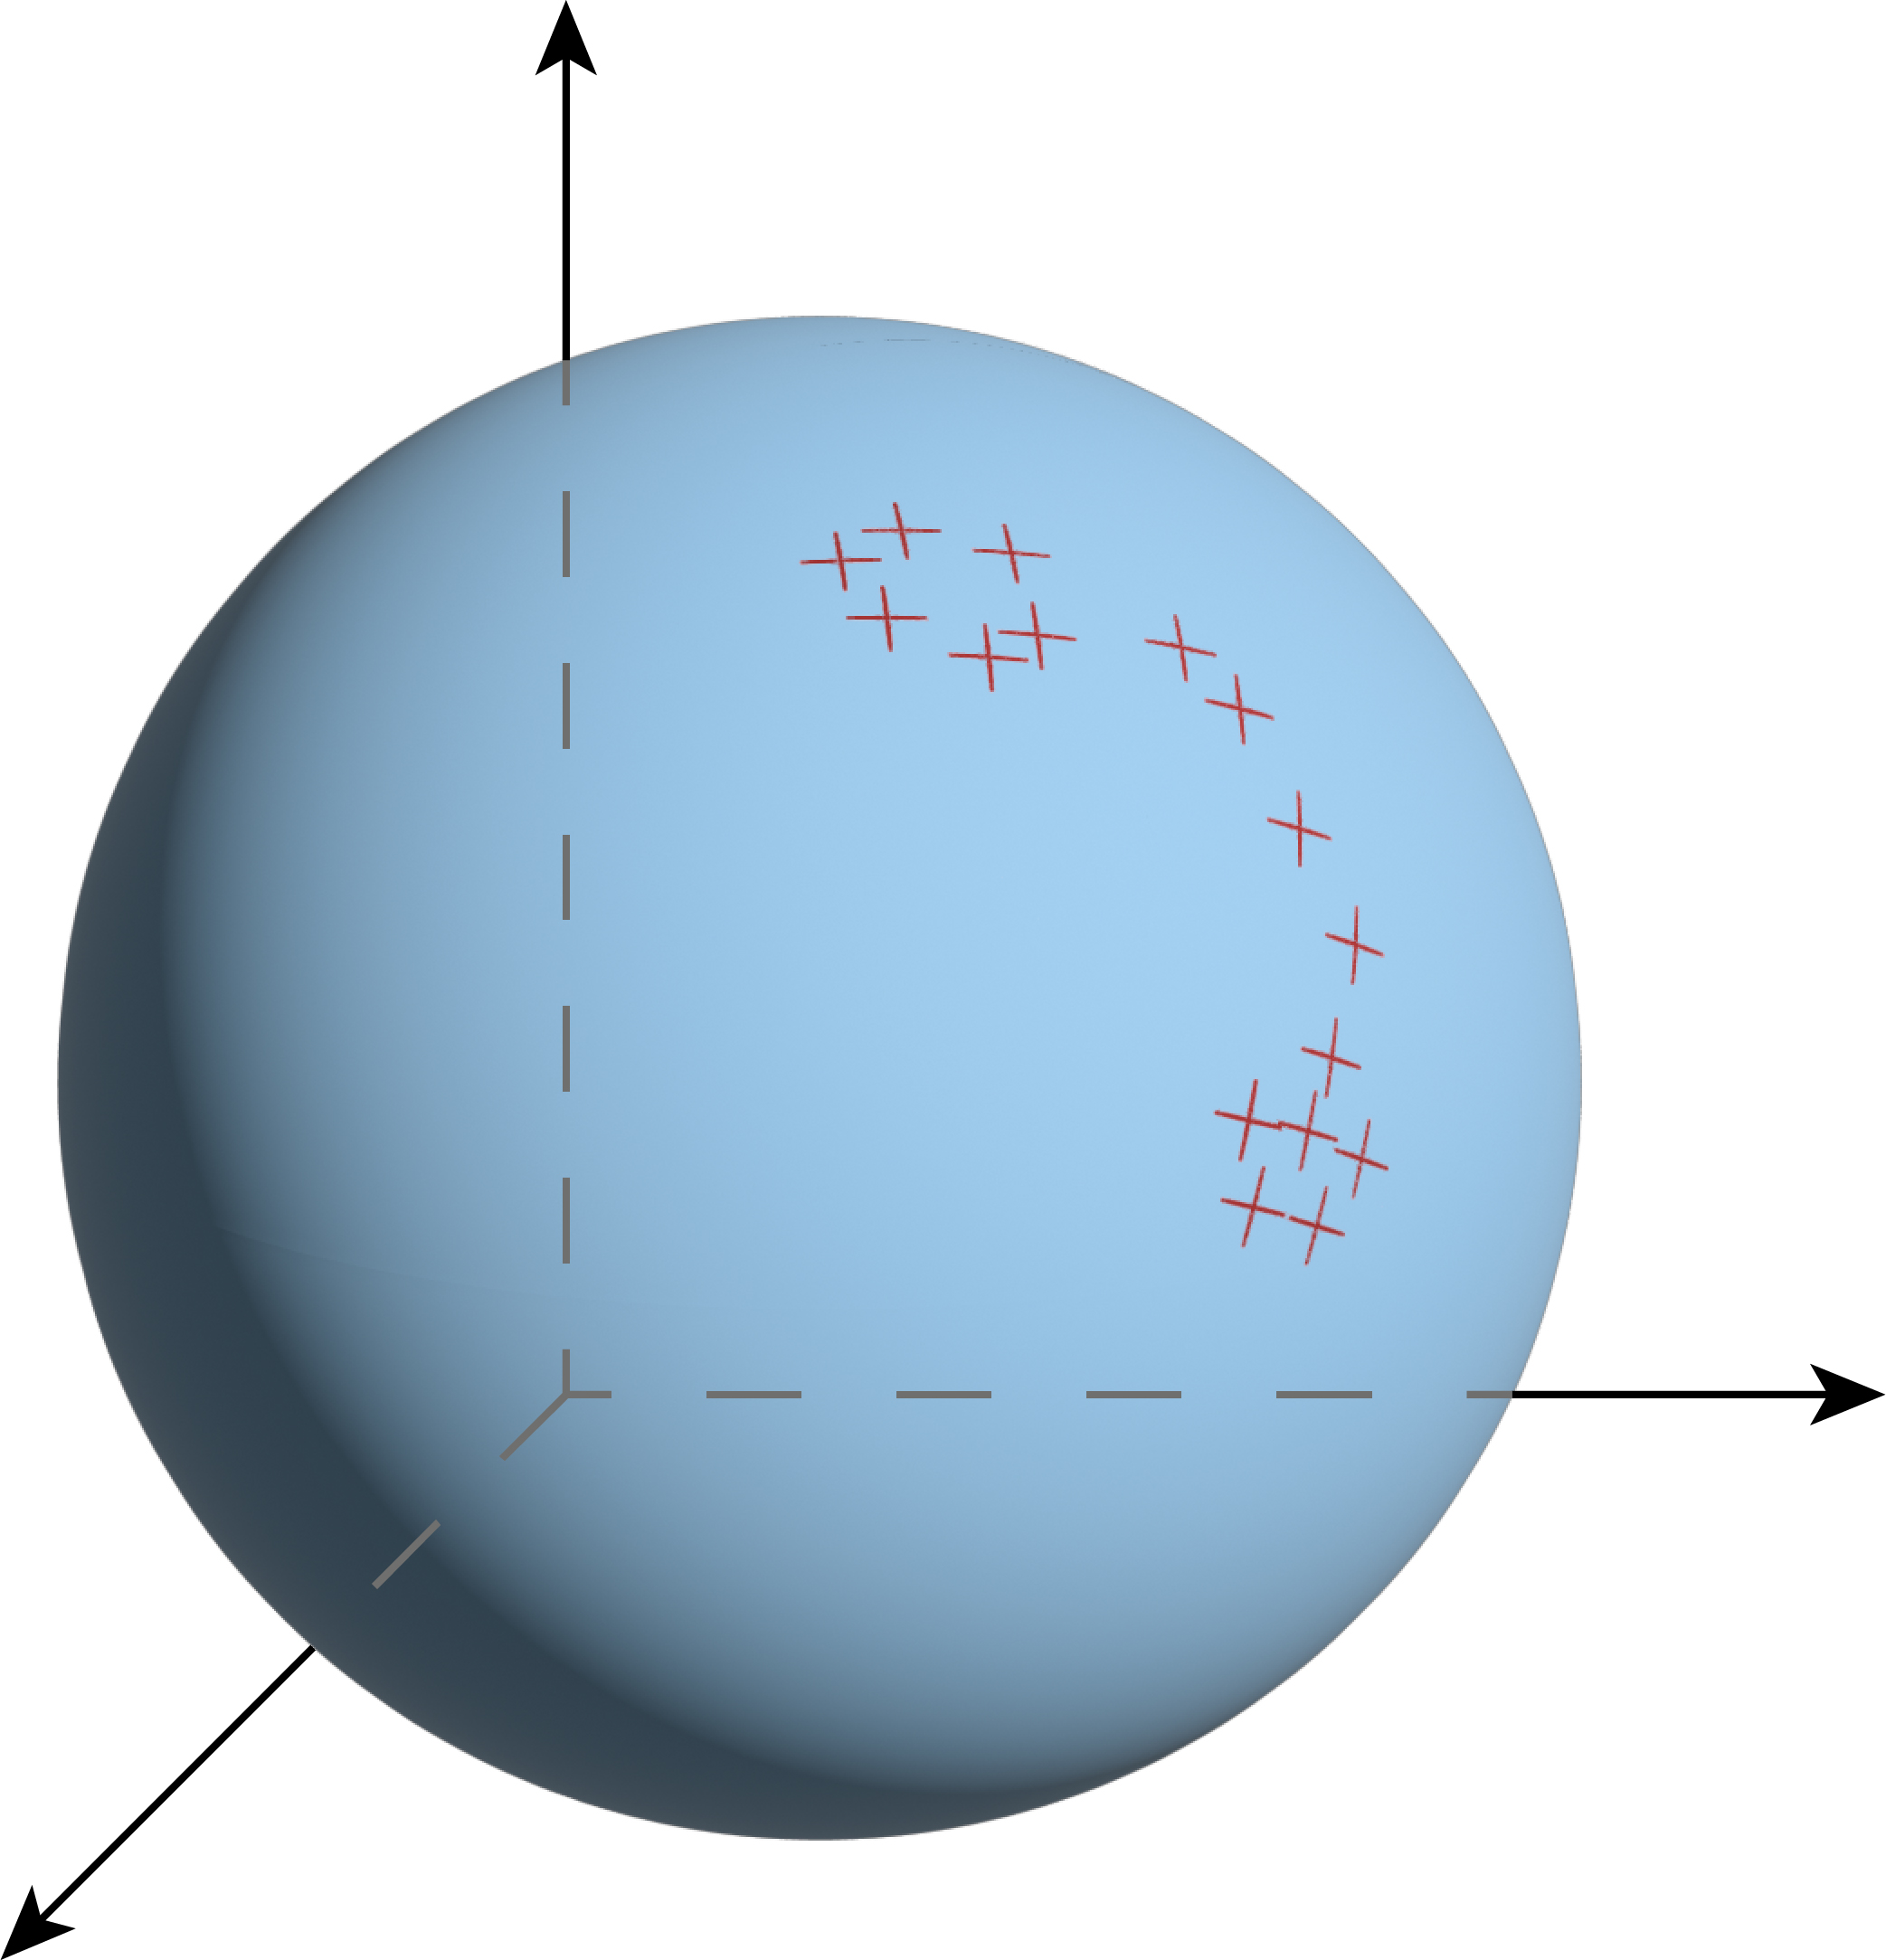
\includegraphics[width=\linewidth]{images/constraind_diffusion_rejection/intro_figure_manifold@600x-100.jpg}
		\caption{\(\c{S}^2\subset\R^3\)}
		\label{fig:intro_figure_manifold}
	\end{subfigure}
	\hfill
	\begin{subfigure}[b]{0.23\textwidth}
		\centering
		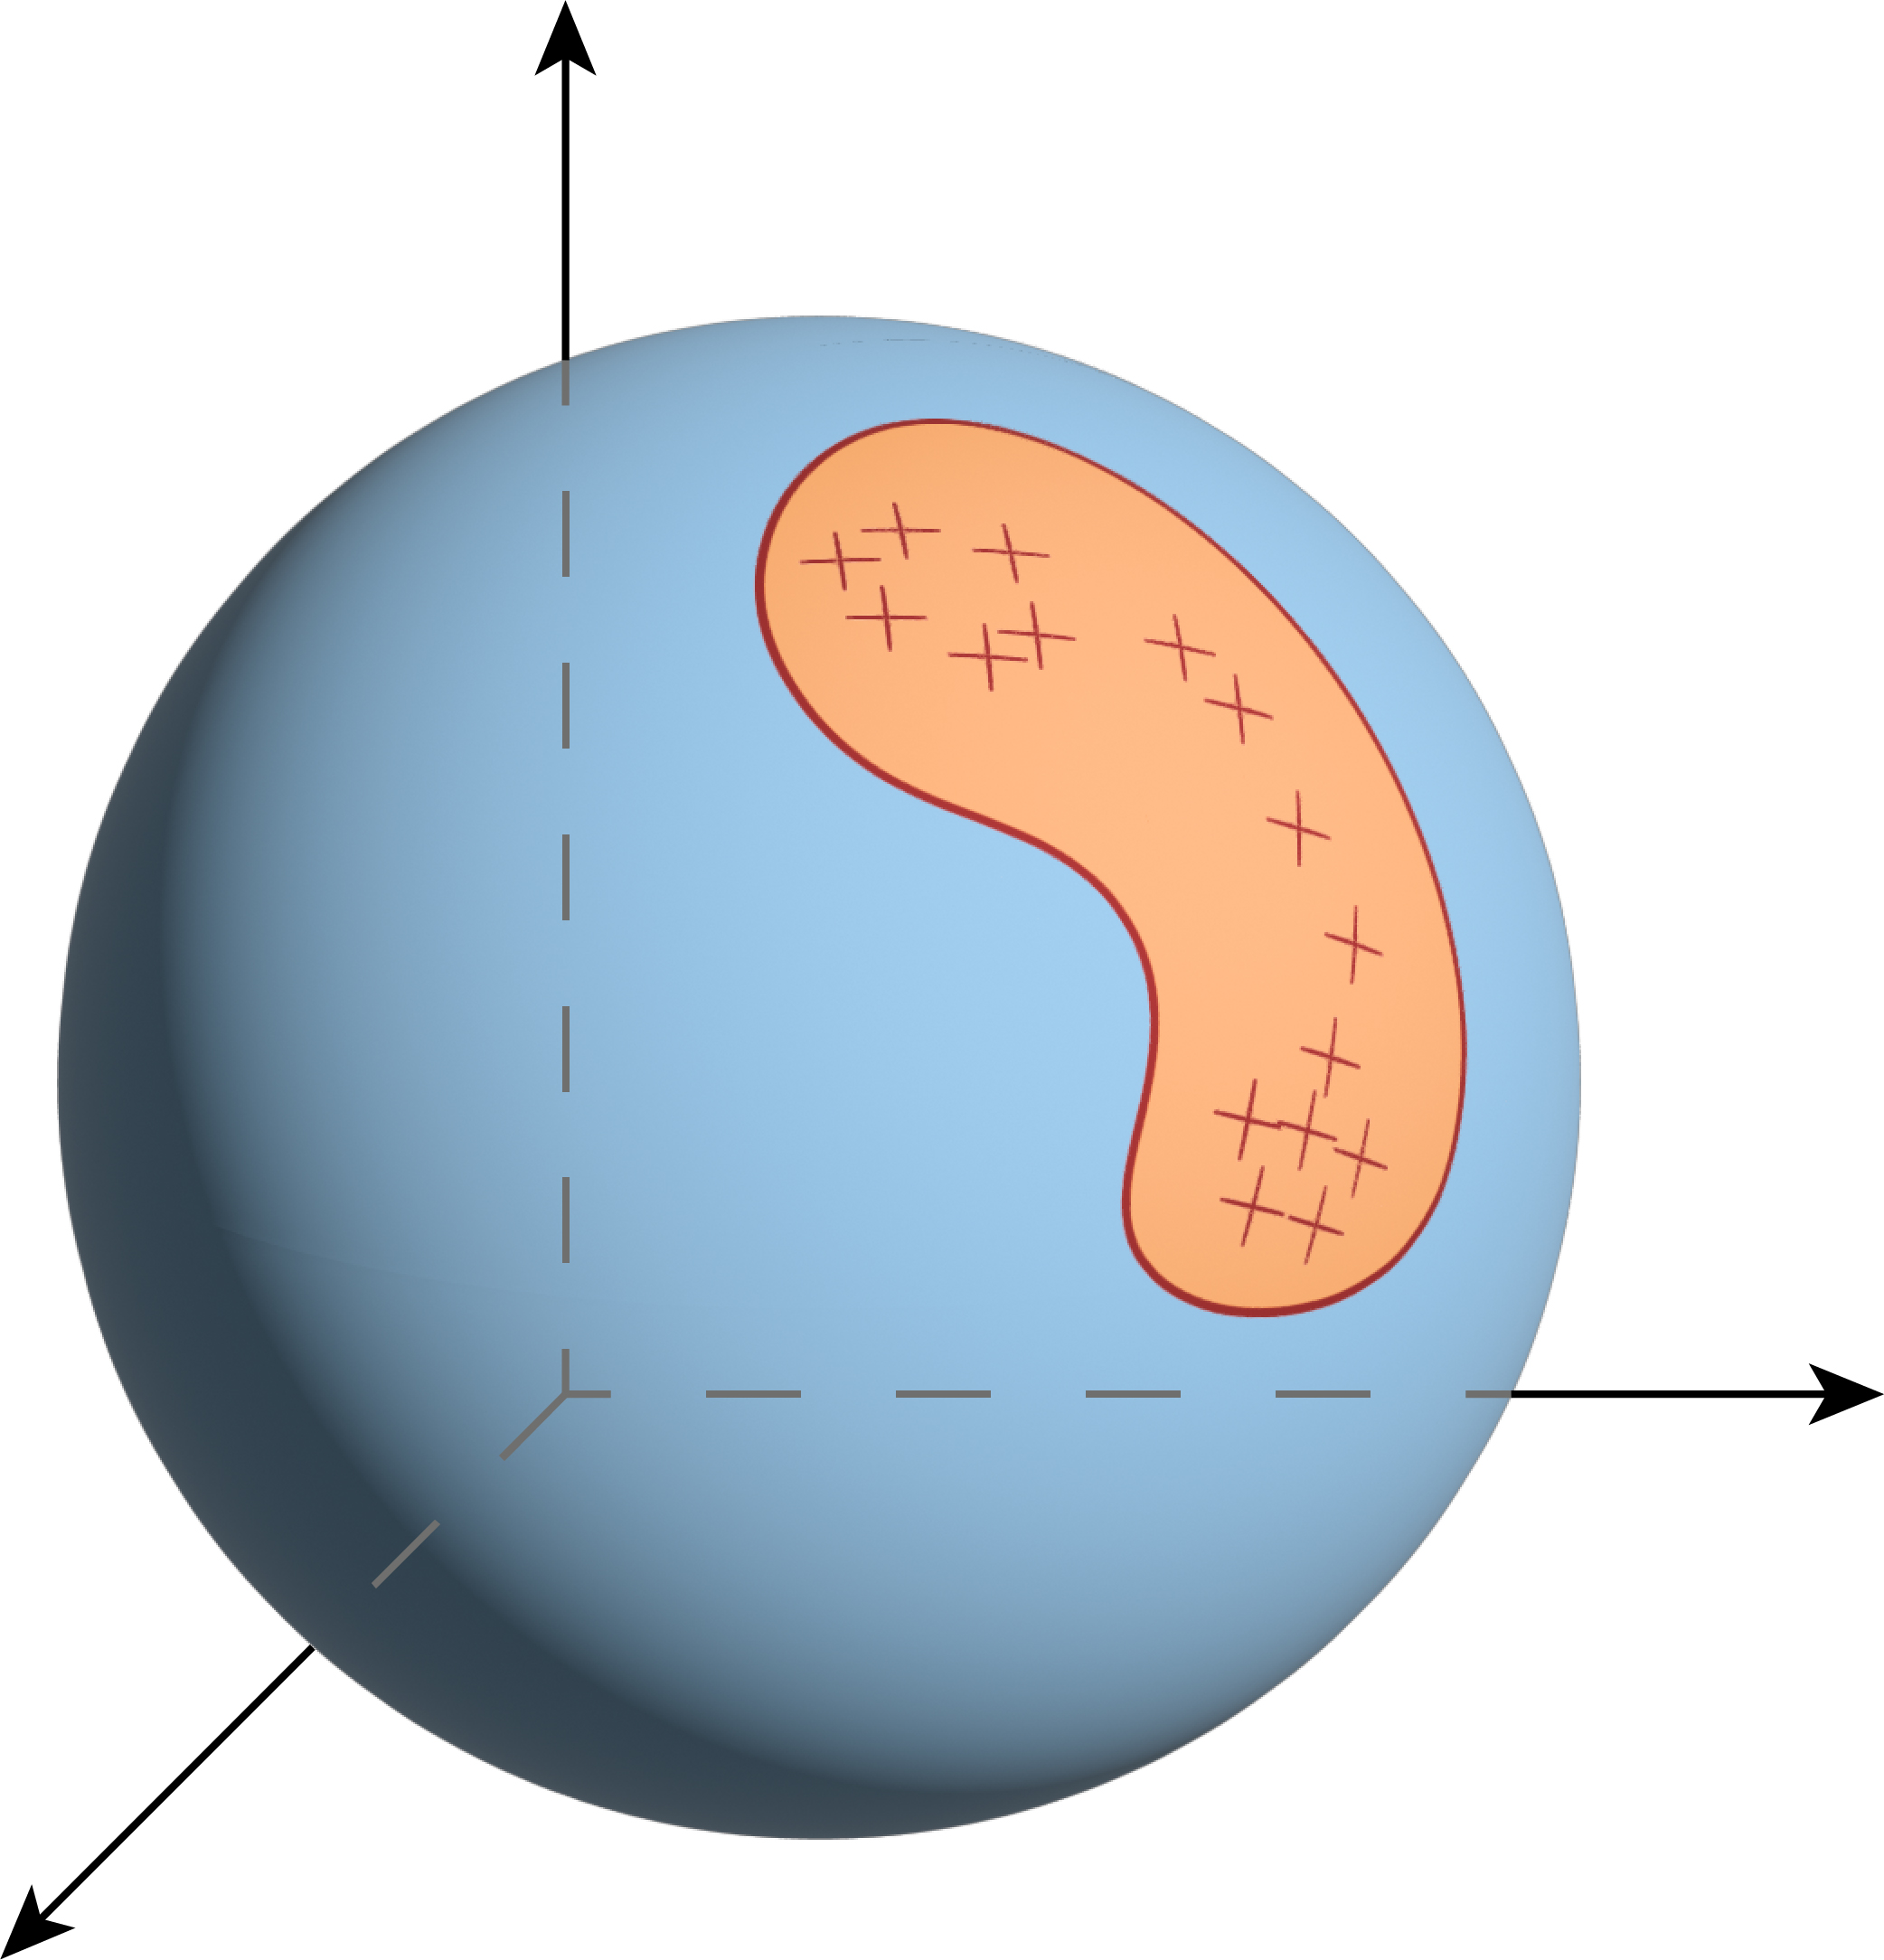
\includegraphics[width=\linewidth]{images/constraind_diffusion_rejection/intro_figure_constrained@600x-100.jpg}
		\caption{\(\c{M}\subset\c{S}^2\subset\R^3\)}
		\label{fig:intro_figure_constrained}
	\end{subfigure}
	\caption{When operating in data-scarce settings, it is often helpful to provide a model with as much prior information about the domain as possible.
		Consider a distribution over a subset \(\c{M}\) of the unit sphere \(\c{S}^2\subset\R^3\).
		While a Euclidean diffusion model can approximate the distribution in \(\R^3\) (a), directly modelling it on \(\c{S}^2\) can make learning significantly easier (b).
		Reducing the problem space even further by only constructing a diffusion model on \(\c{M}\) can lead to even better performance (c).
	}
	\label{fig:intro_figure}
\end{figure}

% In recent years, denoising diffusion models \parencite{sohl2015deep,song2019generative,song2020score,ho2020denoising} have emerged as a powerful paradigm for generative modelling, achieving state-of-the-art performance across a range of domains.
% They work by progressively adding noise to data following a Stochastic Differential Equation (SDE)---the forward \emph{noising} process---until it is close to the invariant distribution of the SDE.
% The generative model is then given by an approximation of the associated time-reversed \emph{denoising} process, which is also an SDE whose drift depends on the gradient of the logarithmic densities of the forward process, referred to as the \emph{Stein score}.

In the previous chapter we extended the framework of score-based genreative modelling to a wide range of Riemannian manifolds, enabling the specification of inherent structural properties of the modelled domain.
This has broadened the applicability of diffusion models to problems in the natural and engineering sciences, including the conformational modelling of small molecules \parencite{jing2022torsional, corso2022DiffDock}, proteins \parencite{trippe2022Diffusion,watson2022Broadly,yim2023se} and robotic platforms \parencite{urain2022se}.

However, in many data-scarce or safety-critical settings, modellers may want to restrict the modelled domain further by specifying problem-informed constraints to make maximal use of limited experimental data or prevent unwanted behaviour \parencite{Morris2002,han2006inverse,Thiele2013,lukens2020practical}.
As illustrated in~\Cref{fig:intro_figure}, such domain-informed constraints can be naturally represented as a \emph{Riemannian manifold with boundary}.
Training diffusion models on such constrained manifolds is thus an important problem that requires principled noising processes---and corresponding discretisations---that stay within the constrained set.

A key assumption of the Riemannian diffusion models introduced in the previous chapter is that the stochastic processes they consider are defined \emph{for all times}.
While this holds for a large class of stochastic processes, it is not the case for most manifolds defined via a set of inequality constraints.
For instance, in the case of the hypercube \(\del{-1,1}^d\) equipped with the Euclidean metric, the Riemannian Brownian motion coincides with the Euclidean \(d\)-dimensional Brownian motion \((\v{B}_t)_{t \in \cbr{0,T}}\) as long as \(\v{B}_t \in \del{-1,1}\).
With probability one, \((\v{B}_t)_{t \geq 0}\) escapes from \(\del{-1,1}\), meaning that the Riemannian Brownian motion is not defined for all times and the frameworks introduced does not apply.

Such constrained manifolds comprise a wide variety of settings---including polytopes and convex sets of Euclidean spaces---and are studied across a large number of disciplines, ranging from computational statistics \parencite{Morris2002}, over robotics \parencite{han2006inverse} and quantum physics \parencite{lukens2020practical}, to computational biology \parencite{Thiele2013}.
Deriving principled diffusion models that are able to operate directly on these constrained manifolds is thus of significant practical importance, as they enable generative modelling in data-scarce and safety-critical settings in which constraints on the modelled domain may reduce the number of degrees of freedom or prevent unwanted behaviour.

As sampling problems on such manifolds are important \parencite{kook2022sampling,heirendt2019creation}, a flurry of Markov chain based methods have been developed to sample from unnormalised densities.
Successful algorithms include the reflected Brownian motion \parencite{williams1987Reflected,petit1997Time,shkolnikov2013Timereversal}, log-barrier methods \parencite{Kannan2009,lee2017Geodesic,noble2022Barrier,kook2022sampling,gatmiry2022convergence,lee2018convergence} and hit-and-run approaches in the case of polytopes \parencite{Smith1984,Lovasz2006}.

In this chapter, we study the generative modelling counterparts of these algorithms through the lens of diffusion models.
Among existing methods for statistical sampling on constrained manifolds, the geodesic Brownian motion \parencite{lee2017Geodesic} and the reflected Brownian motion \parencite{williams1987Reflected} are continuous stochastic processes, and thus well suited for extending the continuous Riemannian diffusion framework developed in the previous chapter to manifolds with boundary and constrained domains.
In particular, we introduce two principled diffusion models for generative modelling on constrained domains based on \begin{enumerate*}[label=(\roman*)] \item the geodesic Brownian motion, leveraging tools from the log-barrier methods, and \item the reflected Brownian motion \end{enumerate*}.
In both cases, we show how one can extend the ideas of time-reversal and score matching to these settings.

These methods have some drawbacks however and can be computationally burdensome and numerically unstable.
They require bespoke implementations for different manifolds and constraints.
Concurrently to the development of our methods, \textcite{lou2023reflected} investigated the use of reflected diffusion models for image modelling.
They focus on the high-dimensional hypercube, as this setting admits a theoretically grounded treatment of the \emph{static thresholding} method which is widely used in image models such as \textcite{saharia2022photorealistic}.
Their method exhibits robust scaling properties and impressive visual results in this framework.
However, the introduced samplers suffer from the same limitations as the log-barrier and reflected Brownian motion approches we disucess for more complex manifolds and constraints beyond the hypercube setting.

Therefore we also propose a new method for generative modelling on constrained manifolds based on a novel Metropolis-based discretisation of the reflected Brownian motion.
The Metropolised process' chief advantage is that it is lightweight: the only additional requirement over those outlined in the previous chapter that is needed to implement a constrained diffusion model is an efficient binary function that indicates whether any given point is within the constrained set.
The Metropolised approximation of the reflected Brownian motion is substantially easier to implement, faster to compute and more numerically stable than the other schemes considered.
A core theoretical contribution is to show that this new discretisation converges to the reflected SDE by using the invariance principle for SDEs with boundary \parencite{stroock1971diffusion}.
To the best of our knowledge, this is the first time that such a process has been investigated.
We demonstrate that our method attains improved empirical results on manifolds with convex and non-convex constraints by applying it to a range of problems from geospatial modelling, robotics and protein design.


\subsection{Constrained manifolds.}
\label{sec:manifold_w_boundary}


\begin{figure}[t]
	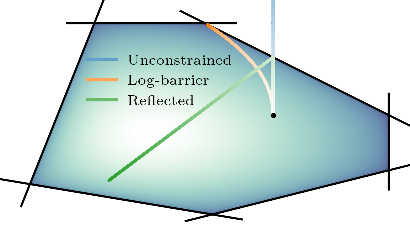
\includegraphics{images/constrained_diffusion/polytope2.pdf}
	\caption{An example of a polytope in two dimensions, with example geodesics under the usual Eucidelan metric, the log-barrier metric, and boundary reflection.}
	\label{fig:polytope}
\end{figure}

In this chapter we are concerned with \emph{constrained} manifolds.
More precisely, given a Riemannian manifold \((\c{N}, g)\), we consider a family of real functions \(\{f_i: \c{N} \to \R\}_{i \in \mathcal{I}}\) indexed by \(\mathcal{I}\).
We then define \begin{equation} \label{eq:constrained} \c{M} = \cbr{x \in \c{N} \; : \; f_i(x) < 0 , \ i \in \mathcal{I}}.
\end{equation}
In this scenario, \(\{f_i\}_{i \in \mathcal{I}}\) is interpreted as a set of constraints on \(\c{N}\).
For example, choosing \(\c{N} = \R^d\) and affine constraints \(f_i(x) = \langle a_i, x\rangle - b_i\), \(x\in \R^d\), we get that \(\c{M}\) is an open polytope as illustrated in \cref{fig:polytope}.
Assuming the constraints together form an open set on the manifold \(c{N}\), we can consider this a \emphhyperref{manifold with boundary}{def:manifold_with_boundary}, \((\c{M}, \partial \c{M}, g)\), and our goal is to model densities that live inside the boundary.
We consider throughout this section that the the constrainst we encounter form a compact set on the manifold.
Many of the results can be extended to the setting of non-compact constraints, but the settings we study do not need this.

This setting naturally appears in many areas of engineering, biology, and physics \parencite{boyd2004convex, han2006inverse, lukens2020practical}.

While the methods we introduce in \Cref{sec:bsgm,sec:reflected_diffusion_model} can be applied to the general framework (\ref{eq:constrained}) , in our applications, we focus on two specific settings: \begin{enumerate*}[label=(\alph*)] \item polytopes---\(\c{N} = \R^d\), \item symmetric positive definite matrices (SPD) under trace conditions---\(\c{N}=\mathcal{S}_{++}^{d}\).
\end{enumerate*}

% \paragraph{Continuous diffusion models.}
% \label{sec:sgm}

% We briefly recall the framework for constructing continuous diffusion processes introduced by \textcite{song2020score} in the context of generative modelling over \(\R^d\).
% At minimum diffusion models need four things: \begin{enumerate*}[label=(\roman*)] \item A forward noising process converging to an invariant distribution.
% 	\item A time reversal for the reverse process.
% 	\item A discretization of the continuous-time process for the forward/reverse process.
% 	\item A score matching loss --- in this paper we will focus on the implicit score matching loss.
% \end{enumerate*}
% \textcite{song2020score} consider a forward \textit{noising process}
% \((\v{X}_{t})_{t \in \cbr{0,T}}\) which progressively noises a data distribution
% \(p_0\) into a Gaussian \(\mathrm{N}(0,\m{I})\).
% More precisely \((\v{X}_{t})_{t \in \cbr{0,T}}\) is an Ornstein–Uhlenbeck (OU) process which is given by the following stochastic differential equation (SDE) \begin{equation} \label{eq:ornstein_uhlenbeck} \mathrm{d} \v{X}_t = - \tfrac{1}{2}\v{X}_t \mathrm{d} t + \mathrm{d} \v{B}_t, \qquad \v{X}_0 \sim p_0.
% \end{equation}
% Under mild conditions on \(p_0\), the time-reversed process \((\overleftarrow{\v{X}}_t)_{t \in \cbr{0,T}} = (\v{X}_{T-t})_{t \in \cbr{0,T}}\) also satisfies an SDE \parencite{cattiaux2021time,haussmann1986time} given by \begin{equation} \label{eq:time_reversal_dupref} \mathrm{d} \overleftarrow{\v{X}}_t = \{\tfrac{1}{2}\overleftarrow{\v{X}}_t + \nabla \log p_{T-t}(\overleftarrow{\v{X}}_t)\} \mathrm{d} t + \mathrm{d} \v{B}_t, \qquad \overleftarrow{\v{X}}_0 \sim p_T, \end{equation} where \(p_t\) denotes the density of \(\v{X}_t\).
% This construction allows direct sampling of the forward process and leverages the Euler-Maruyama discretisation to facilitate sampling of the reverse process.
% Finally, the quantity \(\nabla \log p_t \) is referred as the Stein score and is unavailable in practice.
% It can be approximated with a score network \(s_\theta(t,\cdot)\) trained by minimising a denoising score matching (\(\mathrm{dsm}\)) loss \begin{equation} \label{eq:denoising_sm}  \mathcal{L}(\theta) = \E [ \lambda_t \norm{ \nabla \log p_{t|0}(\v{X}_t|\v{X}_0) - s_\theta(t, \v{X}_t) }^2], \end{equation} or an equivalent score matching (\(\mathrm{ism}\)) loss \begin{equation} \label{eq:implicit_sm} { \mathcal{L}(\theta) = \E[ \lambda_t \{ \tfrac{1}{2} \norm{ s_\theta(t, \v{X}_t) }^2 + \mathrm{div}(s_\theta)(t, \v{X}_t)}\}] + C, \end{equation} where \(C \geq 0\) and \(\lambda_t >0\) is a weighting function, and the expectation is taken over \(t \sim \mathcal{U}([0, T])\) and \((\v{X}_0, \v{X}_t)\).
% For an arbitrarily flexible score network, the global minimiser \(\theta^\star = \mathrm{argmin}_{\theta}\mathcal{L}(\theta)\) satisfies \(s_{\theta^\star}(t, \cdot)=\nabla \log p_t\).

% We are now ready to introduce our methodology to deal with manifolds defined via inequality \emph{constraints} (\ref{eq:constrained_dupref}).
% In \Cref{sec:bsgm}, we propose a Riemannian diffusion model endowed with a metric induced by a log-barrier potential.
% In \Cref{sec:rbm}, we introduce a \emph{reflected} diffusion model.
% While both models extend classical diffusion models to inequality-constrained settings, they exhibit very different behaviours.
% We discuss their practical differences in \Cref{sec:diff_methods}.

\section{Log-barrier diffusion models}
\label{sec:bsgm}

\begin{figure*}[h]
	\begin{minipage}[b]{0.49\textwidth}
		\centering
		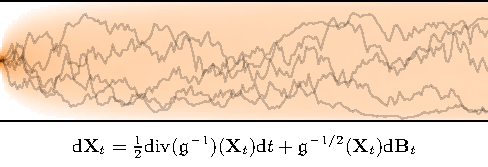
\includegraphics{images/constrained_diffusion/hessian_density.pdf}
		\caption{Convergence of the Barrier Langevin dynamics on the unit interval to the uniform distribution.}
		\label{fig:density}
	\end{minipage}
	\hfill
	\begin{minipage}[b]{0.49\textwidth}
		\centering
		\begin{tikzpicture}
			\tikzset{
				punkt/.style={
						rectangle,
						rounded corners,
						draw=black, very thick,
						text width=9em,
						minimum height=2em,
						text centered},
				pil/.style={
						<->,
						thick,
						shorten <=2pt,
						shorten >=2pt,}
			}
			\node[punkt, text width=6em] (a) at (0,0) {\((\mathcal{N}, h )\)};%
			\node[punkt, text width=6em, right=5em of a] (b) {\((\mathcal{M}, \nabla^2 \phi)\)}
			edge[pil] (a.east);
			\node[draw, above=1em of a] (e) {Original space};
			\node[draw, above=1em of b] (f) {Constrained space};
		\end{tikzpicture}
		\vspace{2.7em}
		\caption{
			Illustrative diagram of the barrier method and the change of metric.
		}
	\end{minipage}
\end{figure*}

\subsection{Barrier Langevin Dynamics.}
Barrier methods work by constructing a smooth potential \(\phi: \c{M} \rightarrow \R\) such that it blows up on the boundary of a desired set, see \textcite{nesterov2018lectures}.
Such potentials are at the basis of interior methods in optimisation \parencite{boyd2004convex}.
Among these functions, the \emph{logarithmic barrier} is the most popular among practitioners ~\parencite{lee2017Geodesic}.

Generically we can define for any \(x \in \c{M}\) \begin{equation} \label{eq:log_barrier_manifold} { \phi(x) = - \sum_{i=1}^m \log(d(x, \partial \c{M}_i)) } \end{equation} 
where \(d(x, \partial \c{M}_i)\) computes the minimum geodesic distance from \(x\) to the boundary \(\partial \c{M}\), made up of the constraints.
In general this is a highly non-trivial optimization problem however.

In special cases we can exploit the constraints at hand to compute this distance function.
For a convex polytope \(\c{M}\) defined by the constraints \(\mathrm{A} x < b\), with \(\mathrm{A} \in \R^{m \times d}\) and \(b \in \R^m\), the logarithmic barrier \(\phi: \ \c{M} \to \R_+\) is given for any \(x \in \c{M}\) by \begin{equation} \label{eq:log_barrier_polytope} { \phi(x) = - \sum_{i=1}^m \log(\langle \mathrm{A}_i, x\rangle-b_i).
	}
\end{equation}
Assuming that \(\| \mathrm{A}_i \| =1\), we have that for any \(x \in \c{M}\), \(\phi(x) = - \sum_{i=1}^m \log(d(x, \partial \c{M}_i))\), where \(\partial \c{M}_i = \cbr{x \in \R^d \; : \; \langle \mathrm{A}_i, x\rangle =b}\).

While developed and most commonly used in optimisation, barrier methods can also be used for sampling \parencite{lee2017Geodesic}.
The core idea of barrier methods is to `warp the geometry' of the constrained space, stretching it as the process approaches the boundary so it never hits it, hence bypassing the need to explicitly deal with the boundary.

Assuming \(\phi\) to be strictly convex and smooth, its Hessian \(\nabla^2 \phi\) is positive definite and thus defines a valid Riemannian metric on \(\c{M}\).
The formal approach to 'warping the geometry' of the convex space with the boundary is to endow \(\c{M}\) with the Hessian as a Riemannian metric \(g = \nabla^2 \phi\), making it into a Hessian Manifold, see \cite{shima1997geometry}.
In the special case where the barrier is given by (\ref{eq:log_barrier_polytope}) , we get for any \(x \in \c{M}\) \begin{equation} g(x) = \mathrm{A}^\top S^{-2}(x) \mathrm{A} \text{ with } S(x) = \text{diag}(b_i - \langle \mathrm{A}_i, x \rangle)_i.
\end{equation}
Equipped with this Riemannian metric, we consider the following Langevin dynamics as a forward process \begin{equation} \label{eq:langevin_hessian_manifold} { \mathrm{d} \v{X}_t^\vsra{} = \tfrac{1}{2} \mathrm{div}(g^{-1})( \v{X}_t^\vsra{}) \mathrm{d} t + g( \v{X}_t^\vsra{})^{-\frac{1}{2}} \mathrm{d} \v{B}_t, } \end{equation} with \(\mathrm{div}(F)(x) \triangleq \left(\mathrm{div}(F_1)(x), \dots, \mathrm{div}(F_d)(x) \right)^\top \), for any smooth \(F: \ \R^d \to \R^d\).

Under mild assumptions on \(\c{M}\), \(\mathrm{div}(g^{-1})\) and \(g^{-1}\) we get that \(( \v{X}_t)_{t \geq 0}\) is well-defined and for any \(t \geq 0\), \( \v{X}_t \in \c{M}\).
In particular, for any \(t \geq 0\), \( \v{X}_t\) does not reach the boundary.
This stochastic process was first proposed by \cite{lee2017Geodesic} in the context of efficient sampling from the uniform distribution over a polytope.
Under similar conditions, \( \v{X}_t\) admits a density \(p_t\) with respect to
the Lebesgue measure and we have that \(\partial_t p_t = \tfrac{1}{2} \mathrm{Tr}(g^{-1} \Delta p_t)\).
In addition, \(( \v{X}_t)_{t \geq 0}\) is irreducible.

Hence, assuming that \(\c{M}\) is compact, the uniform distribution on \(\c{M}\) is the unique invariant measure of the process \(( \v{X}_t)_{t \geq 0}\) and \(( \v{X}_t)_{t \geq 0}\) converges to the uniform distribution in some sense.
A proof of these results is in \Cref{sec:geod-brown-moti}.

\subsection{Time-reversal.}
Assuming that \(g^{-1}\) and its derivative are bounded on \(\c{M}\), the time-reversal of (\ref{eq:langevin_hessian_manifold}) is given by \cref{thm:fokker-plank_time_reversal_manifold}, in particular we have \begin{align} \mathrm{d} \v{X}_t^\vsla{} & = {[-\frac{1}{2} \mathrm{div}(g^{-1}) + \mathrm{div}(g^{-1})} { + g^{-1} \nabla \log p_{T-t} ](\v{X}_t^\vsla{}) \mathrm{d} t + g(\v{X}_t^\vsla{})^{-\frac{1}{2}} \mathrm{d} \v{B}_t,} \\  & = { \left[\frac{1}{2} \mathrm{div}( g^{-1}) + g^{-1} \nabla \log p_{T-t}\right](\v{X}_t^\vsla{}_t) \mathrm{d} t + g(\v{X}_t^\vsla{})^{-\frac{1}{2}} \mathrm{d} \v{B}_t.
                 }  \label{eq:reversal_langevin_hessian_manifold}
\end{align}
\(\v{X}_t^\vsla{}_0\) is initialised with the uniform distribution on \(\c{M}\) (which is close to the one of \( \v{X}_T\) for large \(T\)).

The estimation of the score term \(\nabla \log p_t\) is done by minimising the implicit score-matching loss function (\cref{prop:manifold_ism}) .
We refer to \Cref{sec:score-netw-param} for details on the training and parameterisation.

\subsection{Sampling.}
Sampling from the forward (\ref{eq:langevin_hessian_manifold}) and backward (\ref{eq:reversal_langevin_hessian_manifold}) processes, once the score is learnt, requires a discretisation scheme.
We again use geodesic random walks, \cref{sec:geodesic_random_walk}, for this purpose, see \Cref{alg:grw_cdm}.

In one difference to the previous chapter however, we will not have access explicitly to the exponential map of the Hessian metric.
Instead, we rely on an approximation, using a \emph{retraction} (see \textcite{absil2012projection, boumal2023introduction} for a definition and alternative schemes).

This involves a linear approximation of the exponential map, taking a straight step in the original Euclidean metric, followed by retracting a point back inside the manifold to the closest point inside the constraints if it lies outside them after the step.

\begin{algorithm}[]
	\caption{\emph{Geodesic Random Walk.}
		Discretisation of the SDE \(\mathrm{d} \v{X}_t = d(t, \v{X}_t) \mathrm{d} t + \mathrm{d} \v{B}_t\).
	}
	\label{alg:grw_cdm}
	\begin{algorithmic}[1]
		\Require  \(T\) (simulation time), \(N\) (number of steps), \(X_0^\gamma\) (initial point), \(d\) (drift function)
		\State \(\gamma = T / N\)
		\For{\(k \in \{0, \dots, N-1\}\)}
		\State \(Z_{k+1} \sim \mathrm{N}(0, \m{I})\)
		\State \(W_{k+1} = \gamma d(k \gamma, X_k) + \sqrt{\gamma}
			Z_{k+1}\) 
		\State \(X_{k+1}^\gamma = \exp_{X_k}[W_{k+1}] \approx \mathrm{proj}_\c{M}(X_k + W_{k+1})\) 
		\EndFor 
		\State { \bfseries return} \(\{ X_k\}_{k=0}^{N}\) 
	\end{algorithmic} 
\end{algorithm} 


\section{Reflected diffusion models}
\label{sec:reflected_diffusion_model}
\begin{figure*}[h]
	\label{fig:rbm}
	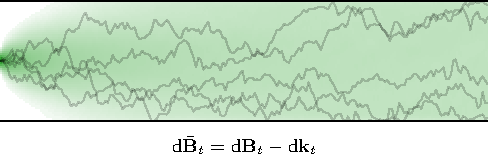
\includegraphics{images/constrained_diffusion/reflected_density.pdf}
	% \hfill
	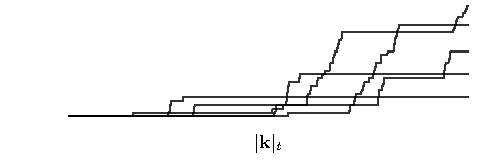
\includegraphics{images/constrained_diffusion/reflected_ks.pdf}
	\caption{\emph{Left:}
		Convergence of the reflected Brownian motion on the unit interval to the uniform distribution.
		\emph{Right:}
		Value of \(\abs{ \v{k}}_t\) for the trajectory samples on the left through time.
	}
\end{figure*}

Another approach to deal with the boundary geometry of \(\c{M}\) is to use the standard metric \(h\) and forward dynamics of \(\c{N}\) and constraining it to \(\c{M}\) by \emph{reflecting} the process whenever it would encounter a boundary.
We will first assume that \(\c{M}\) is compact and convex.
To simplify the presentation we focus on the Euclidean case \(\c{N} = \R^d\) with smooth boundary \(\partial M\)\footnote{We refer to \Cref{sec:time-revers-refl} for a definition of smooth boundary.
}.

The key difference between this approach and the barrier approach is that in the reflected case we leave the geometry unchanged, so all we need to do is show that the dynamics induced by reflecting the forward process whenever it hits the boundary leads to an invariant distribution and admit a time-reversal.

It is worth noting that while barrier approaches have received considerable theoretical attention in the sampling literature \parencite{lee2017Geodesic, noble2022Barrier}, reflected methods have remained comparatively undeveloped from the methodological and practical point of view.
In the next section, we recall the basics of reflected stochastic processes.

\subsection{Skorokhod problem.}
Briefly we intorduce the technical detial needed to define a reflected Brownian motion.
The reflected Brownian motion is defined as the solution to the \emphmarginnote{Skorokhod problem}.
Roughly speaking a solution to the Skorokhod problem consists into two coupled processes \((\bar{ \v{B}}_t, \v{k}_t)_{t \geq 0}\) such that \((\bar{ \v{B}}_t)_{t \geq 0}\) acts \emph{locally} as a Euclidean Brownian motion \(( \v{B}_t)_{t \geq 0}\) and \( \v{k}_t\) compensates for the excursion of \(( \v{B}_t)_{t \geq 0}\) outside the boundary so that \((\bar{ \v{B}}_t)_{t \geq 0}\) remains in \(\c{M}\).

We say that \((\bar{ \v{B}}_t, \v{k}_t)_{t \geq 0}\) is a solution to the \emph{Skorokhod problem} \parencite{skorokhod1961stochastic} if \(( \v{k}_t)_{t \geq 0}\) and \((\bar{ \v{B}}_t)_{t \geq 0}\) are two processes satisfying mild conditions, see \Cref{sec:refl-brown-moti} for a rigorous introduction, such that for any \(t \geq 0\), \begin{equation} \label{eq:rbm} \bar{ \v{B}}_t = \bar{ \v{B}}_0 + \v{B}_t - \v{k}_t \in \c{M}, \end{equation} and \[{\abs{ \v{k}}_t = \int_0^t \mathbf{1}_{\bar{ \v{B}}_s \in \partial \c{M}} \mathrm{d} \abs{ \v{k}_s}}, \quad { \v{k}_t = \int_0^t \v{n}(\bar{ \v{B}}_s) \mathrm{d} \abs{ \v{k}_s} ,}\] where \((\abs{ \v{k}}_t)_{t \geq 0}\) is the total variation of \(( \v{k}_t)_{t \geq 0}\) and \( \v{n}\) is the \emphhyperref{outward normal}{def:outward_pointing} to \(\c{M}\)
% \footnote{We extend the normal \( \v{n}\) to the whole space by letting \( \v{n}(x)=0\) if \(x \not \in \partial \c{M}\).}.

When \((\bar{ \v{B}}_t)_{t \geq 0}\) hits the boundary, the condition \[{ \v{k}_t = \int_0^t \v{n}(\bar{ \v{B}}_s) \mathrm{d} \abs{ \v{k}_s} ,}\] tells us that \(- \v{k}_t\) ``compensates'' for \(\bar{ \v{B}}_t\) by pushing the process back into \(\c{M}\) along the inward normal \(- \v{n}\), while the condition \[{\abs{ \v{k}_t} = \int_0^t \mathbf{1}_{\bar{ \v{B}}_s \in \partial \c{M}} \mathrm{d} \abs{ \v{k}_s}}\] can be interpreted as \( \v{k}_t\) being constant when \((\bar{ \v{B}}_t)_{t \geq 0}\) does not hit the boundary.
As a result \((\bar{ \v{B}}_t)_{t \geq 0}\) can be understood as the continuous-time counterpart to the reflected Gaussian random walk.
The process \(( \v{k}_t)_{t \geq 0}\) can be related to the notion of \emph{local time} \parencite{revuz2013continuous} and quantifies the amount of time \((\bar{ \v{B}}_t)_{t \geq 0}\) spends at the boundary \(\partial \c{M}\).
\textcite[Theorem
	2.1]{lions1984stochastic} ensure the existence and uniqueness of a solution to
the Skorokhod problem.
One key observation is that the event \(\{ \bar{ \v{B}}_t \in \partial \c{M} \}\) has probability zero \parencite[Section 7, Lemma 7]{harrison1987brownian}.
As in the \emph{unconstrained} setting, one can describe the dynamics of the density of \(\bar{ \v{B}}_t\).
\begin{proposition}[Reflected Brownian motion Fokker-Plank equation]
	For any \(t > 0\), the distribution of \(\bar{ \v{B}}_t\) admits a density w.r.t.\
	the Lebesgue measure denoted \(p_t\).
	In addition, we have for any \(x \in \mathrm{int}(\c{M})\) and \(x_0 \in \partial \c{M}\) \begin{equation} \label{eq:heat_eq_rbm} \partial_t p_t(x) = \tfrac{1}{2} \Delta p_t(x) , \quad \partial_{ \v{n}} p_t(x_0) = 0 , \end{equation} where we recall that \(\mathbf{n}\) is the outward normal to \(\c{M}\).
\end{proposition}
\begin{proof}
	\textcite{burdzy2004heat}
\end{proof}

Note that contrary to the unconstrained setting, the heat equation has \emph{Neumann} boundary conditions.
Similarly to the compact Riemannian setting \parencite{saloff1994precise} it can be shown that the reflected Brownian motion converges to the uniform distribution on \(\c{M}\) exponentially fast \parencite{loper2020uniform,burdzy2006traps}, see \cref{fig:rbm}.
Hence, \((\bar{ \v{B}}_t)_{t \geq 0}\) is a candidate for a forward noising process in the context of diffusion models.

\subsection{Time-reversal.}
In order to extend the diffusion model approach to the reflected setting, we need to derive a \emph{time-reversal} for \((\bar{ \v{B}}_t)_{t \in \sbr{0,T}}\).
Namely, we need to characterise the evolution of \((\v{X}_t^\vsla{}_t)_{t \in \sbr{0,T}} = (\bar{ \v{B}}_{T-t})_{t \in \sbr{0,T}}\).
It can be shown that the time-reversal of \((\bar{ \v{B}}_t)_{t \in \sbr{0,T}}\) is also the solution to a Skorokhod problem.

\begin{theorem}[Time reversal of reflected Brownian motion]
	\label{sec:time-reversal-reflected}
	There exist \((\v{k}_t^\vsla{})_{t \geq 0}\) a bounded variation process and a Brownian motion \(( \v{B}_t)_{t \geq0}\) such that \begin{equation} { \v{X}_t^\vsla{} = \v{X}_0^\vsla{} + \v{B}_t + \int_0^t \nabla \log p_{T-s}(\v{X}_s^\vsla{}) \mathrm{d} s - \v{k}_t^\vsla{} .
		}
	\end{equation}
	In addition, for any \(t \in \sbr{0,T}\) we have \begin{equation} \label{eq:skorokhod_reversal} {\abs{ \v{k}_t^\vsla{}} = \int_0^t \mathbf{1}_{\v{X}_t^\vsla{}_s \in \partial \c{M}} \mathrm{d} \abs{ \v{k}_s^\vsla{}} , \quad \v{k}_t^\vsla{} = \int_0^t \v{n}(\v{X}_t^\vsla{}_s) \mathrm{d} \abs{ \v{k}_s^\vsla{}} .
		}
	\end{equation}
\end{theorem}
\begin{proof}
	\Cref{sec:time-revers-refl}.
\end{proof}
The proof follows \textcite{petit1997Time} which provides a time-reversal in the case where \(\c{M}\) is the positive orthant.
It is based on an extension of \textcite{haussmann1986time} to the reflected setting, with a careful handling of the boundary conditions.
In particular, contrary to \textcite{petit1997Time}, we do not rely on an explicit expression of \(p_t\) but instead use the intrinsic properties of \(( \v{k}_t)_{t \geq 0}\).

Informally, \cref{sec:time-reversal-reflected} means that the process \((\v{X}_t^\vsla{})_{t \in \sbr{0,T}}\) satisfies \begin{equation} \label{eq:evolution_Y} \mathrm{d} \v{X}_t^\vsla{} = \nabla \log p_{T-t}(\v{X}_t^\vsla{}) \mathrm{d} t + \mathrm{d} \v{B}_t - \mathrm{d} \v{k}_t^\vsla{} , \end{equation} which echoes the usual time-reversal formula (\ref{eq:time_reversal_manifold}).
In practice, in order to sample from \((\v{X}_t^\vsla{}_t)_{t \in \sbr{0,T}}\), one needs to consider the \emph{reflected} version of the \emph{unconstrained} dynamics \[\mathrm{d} \v{X}_t^\vsla{} = \nabla \log p_{T-t}(\v{X}_t^\vsla{}) \mathrm{d} t + \mathrm{d} \v{B}_t.\]

\subsection{Sampling}
In practice, we approximately sample the reflected dynamics by considering the Markov chain given by \Cref{alg:rrw}.
We refer to \textcite{pacchiarotti1998numerical,bossy2004symmetrized} for weak convergence results on this numerical scheme in the Euclidean setting.

\subsection{Likelihood evaluation}
In the case of a reflected Brownian motion, it is possible to compute an equivalent ODE in order to perform likelihood evaluation.
The associated ODE was first derived in \cite{lou2023reflected}.
The form of the ODE and the proof that it remains in \(\c{M}\) are postponed to \Cref{sec:likel-eval}.

\begin{algorithm}[t]
	\begin{algorithmic}
		\Require \(x \in \c{M}\), \(\v{v} \in \mathrm{T}_x\c{M}\), \(\{f_i\}_{i \in \mathcal{I}}\)
		\State \(\ell \gets \norm{\v{v}}_g\)
		\State \(\v{s} \gets \v{v} / \norm{\v{v}}_g\)
		\While{\(\ell \geq 0\)}
		\State \(d_i = \arg \intersect_t\sbr{\exp_g(x, t\v{s}), f_i}\)
		\State \(i \gets \argmin_i\; d_i \; s.t. \; d_i > 0\)
		\State \(\alpha \gets \min\del{d_i, \ell} \)
		\State \(x' \gets \exp_g\del{x, \alpha\v{s}}\)
		\State \(\v{s} \gets \paralleltransport_g\del{x, \v{s}, x'} \)
		\State \(\v{s} \gets \reflect\del{\v{s}, f_i}\)
		\State \(\ell \gets \ell - \alpha\)
		\State \(x \gets x'\)
		\EndWhile
		\State \textbf{return} \(x\)
	\end{algorithmic}
	\caption{\emph{Reflected step algorithm}.
		The algorithm operates by repeatedly taking geodesic steps until one of the constraints is violated, or the step is fully taken.
		Upon hitting the boundary we parallel transport the tangent vector to the boundary and then reflect it against the boundary.
		We then start a new geodesic from this point in the new direction.
		The \({\arg} \intersect_t\) function computes the distance one must travel along a geodesic in direction \(\v{s}\) til constraint \(f_i\) is intersected.
		For a discussion of \(\paralleltransport\), \(\exp_g\) and \(\reflect\) please see \cref{sec:riemannain_intro_dupref}.
	}
	\label{alg:reflection}
\end{algorithm}

\begin{algorithm}[t]
	\caption{\emph{Reflected Random Walk}.
		Discretisation of the SDE \(\mathrm{d} \v{X}_t = b(t, \v{X}_t) \mathrm{d} t + \mathrm{d} \v{B}_t - \mathrm{d} \v{k}_t\).
	}
	\label{alg:rrw}
	\begin{algorithmic}
		\State { \bfseries Require:} \(T\) (simulation time), \(N\) (number of steps), \(X_0^\gamma\) (initial point), \(\{f_i\}_{i \in \mathcal{I}}\) (boundary functions)
		\State \(\gamma = T / N\)
		\For{\(k \in \{0, \dots, N-1\}\)}
		\State \(Z_{k+1} \sim \mathrm{N}(0, \m{I})\)
		\State \(X_{k+1}^\gamma = \text{ReflectedStep}[X_{k}^\gamma, \sqrt{\gamma}
			Z_{k+1}, \{f_i\}_{i \in \mathcal{I}}]\) \EndFor \State { \bfseries return} \(\{ X_k^\gamma\}_{k=0}^{N}\) \end{algorithmic} \end{algorithm} 

\begin{figure*}[t] \centering \begin{minipage}[0.25\textwidth]{0.25\textwidth} 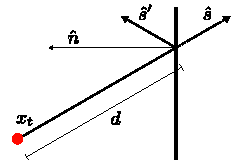
\includegraphics{images/constrained_diffusion/linear_reflection.pdf} \end{minipage} \hfill \begin{minipage}[0.25\textwidth]{0.7\textwidth} \caption{Reflection against a linear boundary.
			For a step \(s\) with magnitude \(|s|\) and direction \(\hat{s}\) the distance to the boundary described by the normal \(\hat{n}\) and offset \(b\) is \(d=\frac{\innerprod{\hat{s}}{x_t} - b}{\innerprod{\hat{s}}{\hat{n}}}\).
			The reflected direction is given by \(\hat{s}' = \hat{s} - 2\innerprod{\hat{s}}{\hat{n}}\hat{n}\).
		}
		\label{fig:reflection_diagrams_lin}
	\end{minipage}
	\vspace{1em}
	\begin{minipage}{0.25\textwidth}
		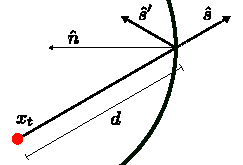
\includegraphics{images/constrained_diffusion/sphere_reflection.pdf}
	\end{minipage}
	\hfill
	\begin{minipage}{0.7\textwidth}
		\caption{Reflection against a spherical boundary.
		For a sphere of radius \(r\), the distance to the boundary from \(x_t\) in direction \(s\) is given by \(d= \frac{1}{2}(\innerprod{\hat{s}}{x_t}^2 + 4 (r^2 - \norm{x_t}^2))^{1/2} -\frac{1}{2}\innerprod{\hat{s}}{x_t}\).
		The normal at the intersection can be computed as the unit vector in the direction \(-2(d\hat{s} + x_t)\), and then \(\hat{s}'\) as above.
		}
		\label{fig:reflection_diagrams_sph}
	\end{minipage}
\end{figure*}

\section{Metropolis sampling of reflected diffusion models}
\label{sec:metropolis_sampling}
Building on the reflected diffusion model intorducted in \cref{sec:reflected_diffusion_model}, we now propose a new discretisation of the reflected Brownian motion that is much cheaper to compute than the typical one previously discussed.

As a reminder, the usual discretisation of the reflected SDE is to \begin{enumerate*}[label=(\roman*)] \item consider a classical step of the Euler-Maruyama discretization (or the Geodesic Random Walk in the Riemannian setting) and \item reflect this step according to the boundary defined by \(\partial \c{M}\).
\end{enumerate*}
To compute the reflection, one must check whether the step crosses the boundary.
If it does, the point of intersection needs to be calculated, the ray reflected at this point, and the step continued in the reflected direction.
This can require an arbitrarily large number of reflections depending on the step size, the geodesic on the manifold, and the geometry of the bounded region within the manifold.

An alternative approach to discretising a reflected SDE is to replace the reflection with a projection, see \cite{slominski1994approximation} for instance.
However, the projection still requires the most expensive part of the reflection algorithm: computing the intersection of the geodesic with the boundary.

Instead of these two approaches, which require manifold and constraint specific functions to be implemented in order to be applied we propose a new sampling scheme based on Metropolis sampling that only requires an indicator function for if the constraint has been violated or not.

The sampler we propose is similar to a classical Euler-Maruyama discretisation of the Brownian motion, except that, whenever a step would carry the Brownian motion outside of the constrained region, we reject it.
This is a \emph{Metropolised} version of the usual discretisation and is almost trivial to implement compared to the existing barrier, reflection and projection methods.
Hence, this method enables the principled extension of diffusion models to arbitrarily constrained domains at virtually {no added implementational complexity or computational expense}.
We call this process the \emphmarginnote{rejection approximation of reflected Brownian motion}.

This is outlined in \cref{alg:metropolis_approx}.
\begin{algorithm}[H]
	\caption{Metropolis approximation of reflected Brownian motion}
	\label{alg:metropolis_approx}
	\begin{algorithmic}
		\Require \(p \in \c{M}\), \(\{f_i\}_{i \in \c{I}}\)
		\State Sample \(\v{v} \sim \mathrm{N}(0,\m{I}) \in \mathrm{T}_p\c{M}\)
		\State \(p' \gets \exp_{p}(\v{v})\)
		\If{\(f_i(p') < 0\ \forall\ i\)}
		\State \(p\gets p'\)
		\EndIf
		\Return \(p\)
	\end{algorithmic}
\end{algorithm}

\subsection{Convergence of the Metropolis sampler to the reflected Brownian motion}
\label{sec:theoretical_convergence}

In this section, we prove that the proposed Metropolis sampling-based process (\cref{alg:metropolis_approx}) corresponds to a valid discretization of the reflected process, \cref{eq:rbm}, justifying its use in diffusion models.
Here we focus on a concise presentation of the core concepts and the main results.
A full proof can be found in \Cref{sec:rejection-convergence}.

For simplicity, we restrict ourselves to the Euclidean setting.\todo{extend to manifold comment?}
All of our results require particular assumptions on \(\c{M}\), which we discuss at the end of this section.
We begin with a definition of the Metropolis approximation of reflected Brownian motion.

\begin{definition}[Metropolis approximation of reflected Brownian motion]
	For any \(\gamma >0\) and \(k \in \N\), let \(X_0^\gamma \in \c{M}\) and \(X_{k+1}^\gamma = X_k^\gamma + \sqrt{\gamma} Z_k^\gamma\) if \(X_k^\gamma + \sqrt{\gamma} Z_k^\gamma \in \c{M}\) and \(X_k^\gamma\) otherwise.
	The sequence \((X_k^\gamma)_{k \in \N}\) is called the \emph{Metropolis approximation of reflected Brownian motion}.
\end{definition}
For any \(\gamma > 0\), we consider \((\v{X}_t^\gamma)_{t \geq 0}\), the linear interpolation of \((X^\gamma_k)_{k \in \N}\) such that for any \(k \in \N\), \(\v{X}_{k \gamma}^\gamma = X_k^\gamma\).
The following result is the main theoretical contribution of this section.

\begin{theorem}[Convergence of the Metropolis approximation to the reflected Brownian motion]
	\label{thm:weak_convergence_metropolis}
	Under assumptions on \(\c{M}\), for any \(T \geq 0\), \((\v{X}_t^\gamma)_{t \in \cbr{0,T}}\) weakly converges to the refelcted Brownian motion \((\bar{\v{B}}_t)_{t \in \cbr{0,T}}\) as \(\gamma \to 0\).
\end{theorem}

The rest of the section is devoted to a high level presentation of the proof of \Cref{thm:weak_convergence_metropolis}.

It is theoretically impractical to work directly with the Metropolis approximation of reflected Brownian motion.
Instead, we introduce an auxiliary process, show this converges to the refelcted Brownian motion, and finally prove that the convergence of the auxiliary process implies the convergence of our Metropolis discretisation.
We define this auxiliary process now.

\begin{definition}[Rejection approximation of reflected Brownian motion]
	For any \(\gamma > 0\) and \(k \in \N\), let \(\hat{X}_0^\gamma = x \in \c{M}\) and \(\hat{X}_{k+1}^\gamma = \hat{X}_k^\gamma + \sqrt{\gamma} Z_k^\gamma\) with \(Z_k^\gamma\) a Gaussian random variable conditioned on \(\hat{X}_k^\gamma + \sqrt{\gamma} Z_k^\gamma \in \c{M}\).
	The sequence \((\hat{X}_k^\gamma)_{k \in \N}\) is called the \emph{rejection approximation of reflected Brownian motion}.
\end{definition}
We call this process the \emph{rejection approximation of reflected Brownian motion} since in practice, \(Z_k^\gamma\) can be sampled using rejection sampling, see~\Cref{alg:rejection_sampling}.
\begin{algorithm}[H]
	\caption{\emph{Rejection approximation of reflected Brownian motion}}
	\label{alg:rejection_sampling}
	\begin{algorithmic}
		\Require \(p \in \c{M}\), \(\{f_i\}_{i \in \c{I}}\)
		\State Sample \(\v{v} \sim \mathrm{N}(0,\m{I}) \in \mathrm{T}_p\c{M}\)
		\State \(p' \gets \exp_{p}(\v{v})\)
		\While{\(f_i(p') \geq 0\ \text{for any}\ i\)}
		\State Sample \(\v{v} \sim \mathrm{Id}(0,1) \in \mathrm{T}_p\c{M}\)
		\State \(p' \gets \exp_{p}(\v{v})\)
		\EndWhile
		\Return \(p'\)
	\end{algorithmic}
\end{algorithm}
The key difference between the rejection and Metropolis approaches is that where the Metropolis approach will leave the point stationary if the update falls outside the boundary, the rejection approach will resample the update until it lies inside the boundary.
While it is possible to implement the rejection approach practially, it is less desirable as it results in loops of unknown length.

For any \(\gamma > 0\), we also consider \((\hat{\v{X}}_t^\gamma)_{t \geq 0}\), the linear interpolation of \((\hat{X}^\gamma_k)_{k \in \N}\) such that for any \(k \in \N\), \(\hat{\v{X}}_{k \gamma}^\gamma = \hat{X}_k^\gamma\).
In~\Cref{sec:rejection-convergence}, we prove the following result.

\begin{theorem}[Convergence of the rejection approximation to the reflected Brownian motion]
	\label{thm:weak_convergence_rejection}
	Under assumptions on \(\c{M}\), for any \(T \geq 0\), \((\hat{\v{X}}_t^\gamma)_{t \in \cbr{0,T}}\) weakly converges to the reflected Brownian motion \((\bar{\v{B}}_t)_{t \in \cbr{0,T}}\) as \(\gamma \to 0\).
\end{theorem}

\begin{proof}
	See \cref{sec:rejection-convergence}.

	Here we give some elements of the proof.
	Our approach is based on the invariance principle of \cite{stroock1971diffusion}.
	More precisely, we show that we can compute an equivalent `drift' and `diffusion matrix' for the discretised process and that, as \(\gamma \to 0\), the drift converges to zero and the diffusion matrix converges to \(\m{I}\).

	In the Euclidean setting, this result, accompanied by mild regularity and growth assumptions, ensures that the discretization weakly converges to the original SDE.
	However, the case with boundary is much more complicated, primarily because the approximate drift might explode near the boundary, thus we need to verify exactly how the drift behaves as \(\gamma \to 0\) and as the process approaches the boundary.

	We show that the \emph{normalised} drift converges to the inward normal near the boundary.
	This ensures that \begin{enumerate}[label=(\alph*)] \item in the interior of \(\c{M}\) the drift converges to zero, i.e.~locally in the interior of \(\c{M}\) the Brownian motion and the reflected Brownian motion coincide, \item on the boundary, the drift pushes the samples inside the manifold according to the inward normal, mimicking \((\v{k}_t)_{t \geq 0}\) in \eqref{eq:rbm_dupref}.
	\end{enumerate}
	Finally, with results from \cite{stroock1971diffusion} and \cite{kang2017submartingale}, we show the convergence to the reflected Brownian motion.

\end{proof}

Our next step is to show that the approximate drift and diffusion matrix of the Metropolised process are upper and lower bounded by their counterparts in the rejection process.
While the upper-bound is easy to derive, the lower-bound requires the following result.

\begin{proposition}
	\label{lemma:lower_bound_prob_main}
	Under assumptions on \(\c{M}\), \(\forall \; \varepsilon > 0\), \(\exists \; \bar{\gamma} >0\) such that for any \(\gamma \in \del{0, \bar{\gamma}}\) and for any \(x \in \c{M}\), \(\gamma \in \del{0, \bar{\gamma}}\) and \(Z \sim \mathrm{N}(0, \m{I})\) we have \(\mathbb{P}(x + \sqrt{\gamma} Z \in \c{M}) \geq 1/2-\varepsilon\), with \(Z \sim \mathrm{N}(0, \m{I})\).
\end{proposition}

\Cref{lemma:lower_bound_prob_main} tells us that \emph{locally} the boundary
looks like a half-space when integrating w.r.t. a Gaussian measure.
A corollary is that, for \(\gamma > 0\) small enough and for any \(k \in \N\), the probability that \(X_{k+1}^\gamma = X_k^\gamma\) is upper bounded \emph{uniformly} w.r.t.
\(X_k^\gamma \in \c{M}\).
The proof of \cref{lemma:lower_bound_prob_main} uses \cref{thm:tubul-neighb} in~\Cref{sec:rejection-convergence}, whose proof relies on the concept of \emph{tubular neighborhoods} \parencite{lee2013smooth}.\todo{background tubular neighbourhoods}

Having established the lower and upper bound, we can conclude the proof by noting that the approximate drift and the diffusion matrix in the rejection and Metropolis case coincide as \(\gamma \to 0\).
This is enough to apply the same results as before, giving the desired convergence.

\paragraph{Assumptions on \(\c{M}\).}
Before concluding this section, we detail the assumptions we make on \(\c{M}\).
For \cref{thm:weak_convergence_metropolis} to hold, we assume that \(\c{M} = \cbrcolon{x \in \R^d}{\Phi(x) > 0}\) is bounded, with \(\Phi \in \c{C}^2(\R^d, \R)\) concave.
We have that \(\partial \c{M} = \cbrcolon{x \in \R^d}{\Phi(x) = 0}\).
In addition, we assume that for any \(x \in \partial \c{M}\), \(\norm{\nabla \Phi(x)} = 1\).

These assumptions match those \cite{stroock1971diffusion} use for their study of the existence of solutions to the refelcted Brownian motion.
While it seems possible to relax the \emph{global} existence of \(\Phi\) to a \emph{local} one, the regularity assumption of the domain is key.
This regularity is essential to establish \cref{lemma:lower_bound_prob_main} and the associated geometrical result on tubular neighborhoods.
We also emphasize that the smoothness of the domain is central in the results of \cite{kang2017submartingale} on the equivalence of two definitions of reflected Brownian motion which we rely on.

\section{Training and parametrising constrained score-based diffusion models}
\label{sec:score-netw-param}

The score term \(\nabla \log p_{T-t}\) appearing in both time-reversal processes (\ref{eq:reversal_langevin_hessian_manifold}) and (\ref{eq:evolution_Y}) is intractable.
It is thus approximated with a \emph{score network} \(s_\theta(t, \cdot) \approx \nabla \log p_t\).
We use a multi-layer perceptron architecture with \(\sin\) activation functions, see \cref{sec:exp_details} for more details on the experimental setup.
Due to boundary condition (\ref{eq:heat_eq_rbm}), the normal component of the score is zero at the boundary in the reflected case.

In order to train log-barrier and reflected diffusion models we prove that we can use a \emph{tractable} score matching loss in constrained manifolds.
We will prove that the implicit score-matching loss leads to the recovery of the correct score when we have a boundary, so long as we enforce that the score is zero on the boundary.
This proof holds for both the log-barrier and the reflected process.

\begin{proposition}[Implicit score matching with boundary]
	\label{thm:implicit_score_matching_boundary}
	Let \(s \in \mathrm{C}^\infty(\cbr{0,T} \times \R^d, \R^d)\) such that for any \(x \in \partial \c{M}\) and \(t \geq 0\), \(s_t(x) =0\).
	Then, there exists \(C >0\) such that \begin{equation} {\E\sbr{\norm{\nabla \log p_t - s_t}^2} = \E\sbr{\norm{s_t}^2 + 2~ \mathrm{div}(s_t)}} + C , \end{equation} where \(\mathbb{E}\) is taken over \(\v{X}_t \sim p_t\) and \(t \sim \mathcal{U}([0,T])\).
\end{proposition}
\begin{proof}
	\Cref{app:proof_for_ism}
\end{proof}
This result immediately implies we can optimise the score network using the implicit score matching loss function so long as we enforce a Neumann boundary condition.

Following \cite{liu2022estimating} we can accommodate this in our score parameterisation by additionally scaling the score output of the neural network by a monotone function \(h(d(x, \partial \c{M}))\) where \(d\) is the distance from \(x\) to the boundary, where \(h(0) = 0\).
In particular we use a clipped ReLU function: \(s_\theta(t, x) = \min(1, \textrm{ReLU}(d(x, \partial \c{M}) - \delta)) \cdot \textrm{NN}_\theta(t, x)\) with \(\delta>0\) a threshold so the model is forced to be zero ``close'' to the boundary as well as exactly on the boundary, see \Cref{sec:exp_details} for an illustration.
The inclusion of this scaling function is necessary to produce reasonable results as we show in \cref{sec:boundary_score}. The weighting function in (\ref{eq:implicit_sm}) is set to \(\lambda_t = (t + 1)\).

The forward processes (\ref{eq:langevin_hessian_manifold}) and (\ref{eq:rbm}) for the barrier and reflected methods cannot be sampled in closed form, so at training time samples from the conditional marginals \(p(\v{X}_t|\v{X}_0)\) are obtained by discretising these processes.
In order to take the most of this computational overhead, we use several samples from the discretised forward trajectory \((\v{X}_{t_1}, \cdots, \v{X}_{t_k}|\v{X}_0)\) instead of only using the last sample.

\section{Related Work}

\subsection{Sampling on constrained manifolds.}
Sampling from a distribution on a space defined by a set of constraints is an important ingredient in several computational tasks, such as computing the volume of a polytope \parencite{lee2017Geodesic}.
Incorporating such constraints inside MCMC algorithms while preserving fast convergence properties is an active field of research \parencite{kook2022sampling,lee2017Geodesic,noble2022Barrier}.
In this work, we are interested in sampling from the uniform distribution defined on the constrained set in order to define a proper \emph{forward process} for our diffusion model.
Log-barrier methods such as the Dikin walk or Riemannian Hamiltonian Monte Carlo \cite{Kannan2009,lee2017Geodesic,noble2022Barrier} change the geometry of the underlying space and define stochastic processes which never violate the constraints, see \cite{Kannan2009,noble2022Barrier} for instance.
If we keep the Euclidean metric, then \emph{unconstrained} stochastic processes might not be well-defined for all times.
To counter this effect, it has been proposed to \emph{reflect} the Brownian motion \cite{williams1987Reflected,petit1997Time,shkolnikov2013Timereversal}.
Finally, we also highlight hit-and-run approaches \parencite{Smith1984,Lovasz2006} which generalise Gibbs' algorithm and enjoy fast convergence properties provided that one knows how to sample from the one-dimensional marginals.

\subsection{Diffusion models on manifolds.}
\textcite{debortoli2022riemannian} extended the work of \textcite{song2020score} to
Riemannian manifolds by defining forward and backward stochastic processes in
this setting.
Concurrently, a similar framework was introduced by \textcite{huang2022riemannian} extending the maximum likelihood approach of \textcite{huang2021variational}.
Existing applications of denoising diffusion models on Riemannian manifolds have been focused on well-known manifolds for which one can find metrics so that the framework of \textcite{debortoli2022riemannian} applies.
In particular, on compact Lie groups, geodesics and Brownian motions can be defined in a canonical manner.
Their specific structure can be leveraged to define efficient diffusion models \cite{yim2023se}.
\textcite{leach2022denoising} define diffusion models on
\(\groupSO{3}\) for rotational alignment, while \textcite{jing2022torsional}
consider the product of tori for molecular conformer
generation. \textcite{corso2022DiffDock} use diffusion models on
\(\R^3 \times \groupSO{3} \times \groupSO{2}\) for protein docking
applications.
RFDiffusion \parencite{watson2022Broadly} and FrameDiff also incorporate \(\groupSE{3}\) diffusion models.
Finally, \textcite{urain2022se} introduce a methodology for \(\groupSE{3}\) diffusion models with applications to robotics.

\subsection{Approximation schemes of reflected SDEs}
Several schemes have been introduced to approximately sample from reflected Stochastic Differential Equations.
They can be interpreted as modifications of classical Euler-Maruyama schemes used to discretise SDEs without boundary.
One of the most common approaches is to use the Euler-Maruyama discretisation and project the solution onto the boundary if it escapes from the domain \(\c{M}\).
In this case, mean-square error rates of order \emph{almost} \(1/2\) have been proven under various conditions \parencite{liu1995discretization,chitashvili1981strong,pettersson1995approximations,slominski1994approximation}.
Concretely this means that \(\E[\| \bar{\v{B}}_{t} - X_{n}^{t/n}\|^2] = O(n^{-1+\varepsilon})\) with \(\varepsilon>0\) arbitrary small and where \((X_k^\gamma)_{k \in \N}\) is the projection scheme.

The rate \(1/2\) is tight \parencite{pacchiarotti1998numerical}.
It is possible to use the Euler-Peano method to get slight improvements for a mean-square error rate of order of \(1/2\), but this is impractical as it assumes that one can solve a (simplified) Skorokhod problem, which is usually intractable.

\textcite{liu1993numerical} introduced a \emph{penalised}
method which pushes the solution away from the boundary and shows a mean-square error
of order \(1/4\), see also \cite{pettersson1997penalization}.
Weak errors of order \(1\) have been obtained in \cite{bossy2004symmetrized} and \cite{gobet2001euler} by introducing a reflection component in the discretisation or using some local approximation of the domain to a half-space.
We refer to \cite{pilipenko2014introduction} for an introduction to the discretisation of reflected SDEs.
Closer to our work, \cite{burdzy2008discrete} consider three different methods to approximate reflected Brownian motions on general domains (two based on discrete methods and one based on killed diffusions).
Only qualitative results are provided.
To the best of our knowledge, no previous work in the probability literature has investigated the \emph{Metropolised} scheme we propose.

Our Metropolis scheme is also related to the ball walk \parencite{applegate1991sampling}, which replaces the Gaussian random variable with a uniform over the ball (or the Dikin ellipsoid).
\textcite{applegate1991sampling} and \cite{lovasz2007geometry} have
studied the asymptotic convergence rate of the ball walk, but, to the best of our
knowledge, its limiting behaviour when the step size goes to zero has not been
investigated.

\subsection{Comparison with \cite{lou2023reflected}.}
We now discuss a few key differences between our work and the reflected diffusion models presented in \cite{lou2023reflected}.
First, in the hypercube setting, our methodologies are identical from a theoretical viewpoint.
The main difference is that \cite{lou2023reflected} use an approximation version of the DSM loss (\ref{eq:denoising_sm}) whereas we rely on the ISM loss (\ref{eq:implicit_sm}).
\textcite{lou2023reflected} exploit the specific factorised structure of the hypercube to make the DSM loss tractable, leading to significant practical advantages.
These can however be directly employed in our framework for reflected models, and also in the log-barrier setting.
Second, in our work, we target scientific applications where the underlying geometry is not Euclidean, whereas \cite{lou2023reflected} focus on the case where the constrained domain of interest is the hypercube (a subset of Euclidean space) with image applications, or where the domain can be easily projected into the hypercube, such as the simplex.
Our approach is designed to handle a wider range of settings, such as non-convex polytopes in Euclidean space, or non-Euclidean geometries.

\section{Experimental Results}
\label{sec:exp_constrained}
To demonstrate the practical utility of the methods described in \cref{sec:bsgm,sec:reflected_diffusion_model,sec:metropolis_sampling} we evaluate them on a series of increasingly difficult tasks: synthetic polytopes, modelling of distributions on constrained robotic arms, modelling proteins with loop constraints, and modelling distributions supported inside the highly complex borders of countries on the Earth.

In particular the manifolds and constraints considered are: \1 \([0,1]^d \subset \R^d\), the hypercube embedded in Euclidean space.
\2 The \(d\)-dimensional simplex, embedded in \(\R^{d-1}\).
\3 \(\groupSPD\) the group of \(d\)-dimension positive definite matrices, along with an additional a trace constraint, \(\cbrcolon{\tr\del{m} < C}{m\in \groupSPD}\).
\4 \(c \subset \c{S}^2\), where \(c\) is country on the surface of the Earth, approximated as the 2-sphere.
\0

Unless otherwise stated, all experiments were performed with a 6 layer MLP with \(\sin\) activations, and a forcing term as described in \cref{sec:score-netw-param} to set the score to zero at the boundary smoothly.

\subsection{Synthetic polytopes}
\label{sec:exp_constrained_polytopes}

In this section we explore applying the described methods to the hypercube of various dimensions, and the simplex of various dimensions.
The \(d\)-dimension hypercube is the product of \([0,1]\) intervals \(d\) times, which can be modelled as a subset of Euclidean space as \[\cbrcolon{0\leq x_i\leq 1 \forall i}{\v{x} \in \R^d}.\]

The \(d\)-dimension simplex is defined by \[\cbrcolon{\sum_{i=1}^d x_i = 1}{\v{x}\in \R^d}.\]
This can be parametrised as \[\cbrcolon{\sum_{i=1}^{d-1} x_i \leq 1}{\v{x}\in \R^{d-1}},\] with the final coordinate implicitly defined as \(x_d = 1 - \sum_{i=1}^{d-1} x_i\).
This second form is computationally easier to apply our framework to, and is used in the experiments.

First we compare the log barrier, reflected and metropolised methods to a normal Euclidean score based model.
We train the models on simple bimodal synthetic data on the hypercube and the simplex, and compare the results visually in \cref{fig:synthetic_hypercube,fig:synthetic_simplex} and using the MMD distance \parencite{gretton2012kernel} between the data distribution and the learnt distribution in \cref{tab:synthetic_polytope_mmd}.

We observe that all the proposed methods recover the data distribution on the two-dimensional hypercube and simplex, although the log barrier method visually tends to leave too much mass stuck to the boundary of the manifold.
We also observe that the reflected method consistently yields better results than the log-barrier one as we scale with dimension.

We also note that the Euclidean models are outperformed by the constrained models in lower dimensions, but generate better results in higher dimensions.
There are a number of potential explanations for this: First, we note that the mixture of Normal distributions we use as a synthetic data-generating process places significantly less probability mass near the boundary as its dimensionality increases, more closely resembling an unconstrained mixture distribution that is easier for the Euclidean diffusion models to learn, while posing a challenge to the log-barrier and reflected diffusion models that initialise at the uniform distribution within the constraints.
Additionally, we note that the design space and hyperparameters used for all experiments were informed by best practices for Euclidean models that may be suboptimal for the more complex dynamics of constrained diffusion models.
We do however observe that the Euclidean models place less of their samples within the constraints as dimension increases, defeating the purpose of constrained modelling.

\begin{figure*}[t]
	\label{fig:synthetic_hypercube}
	\centering
	\begin{subfigure}{.195\textwidth}
		\centering
		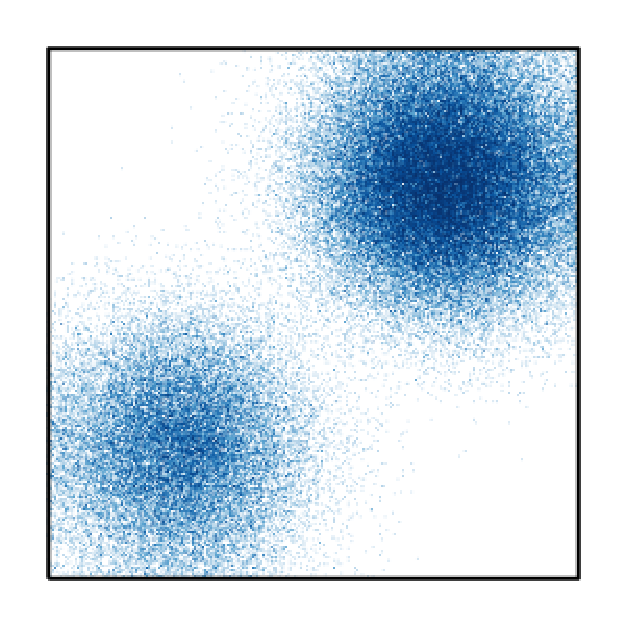
\includegraphics[width=\textwidth]{images/constraind_diffusion_rejection/synthetic_data/synthetic_hypercube_2d_data.pdf}
		\caption{Data distribution}
		\label{fig:synthetic_hypercube_data}
	\end{subfigure}
	\hfill
	\begin{subfigure}{.195\textwidth}
		\centering
		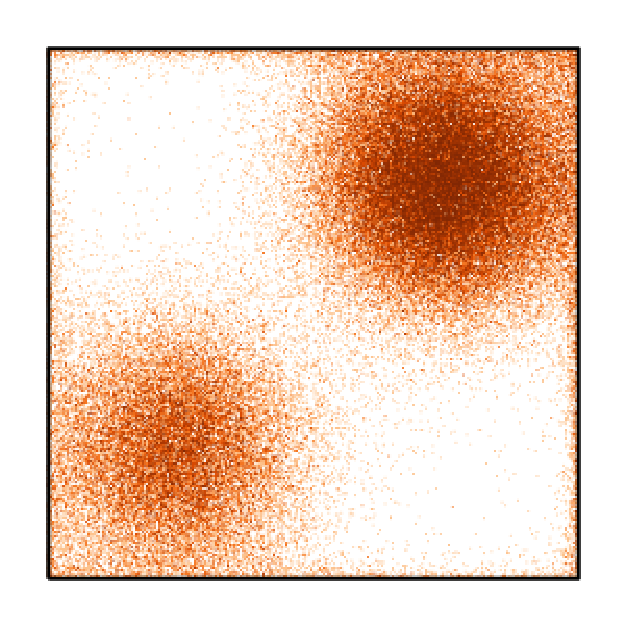
\includegraphics[width=\textwidth]{images/constraind_diffusion_rejection/synthetic_data/synthetic_hypercube_2d_logbarrier.pdf}
		\caption{Log-barrier model}
		\label{fig:synthetic_hypercube_log-barrier}
	\end{subfigure}
	\hfill
	\begin{subfigure}{.195\textwidth}
		\centering
		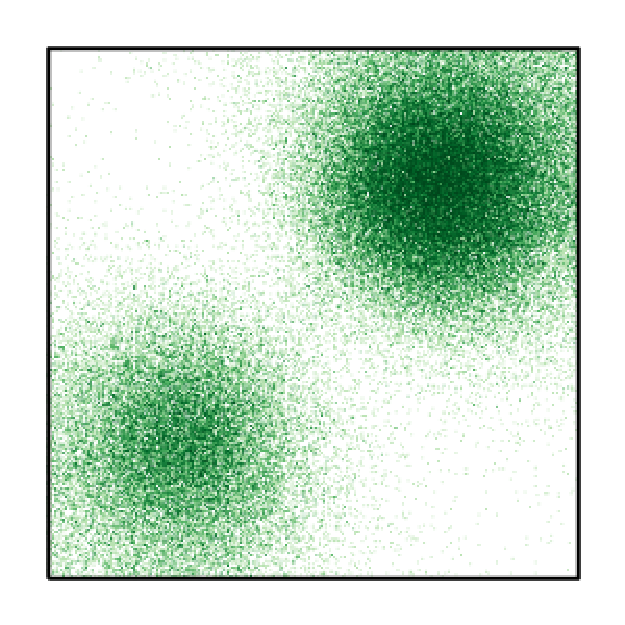
\includegraphics[width=\textwidth]{images/constraind_diffusion_rejection/synthetic_data/synthetic_hypercube_2d_reflected.pdf}
		\caption{Reflected model}
		\label{fig:synthetic_hypercube_reflected}
	\end{subfigure}
	\hfill
	\begin{subfigure}{.195\textwidth}
		\centering
		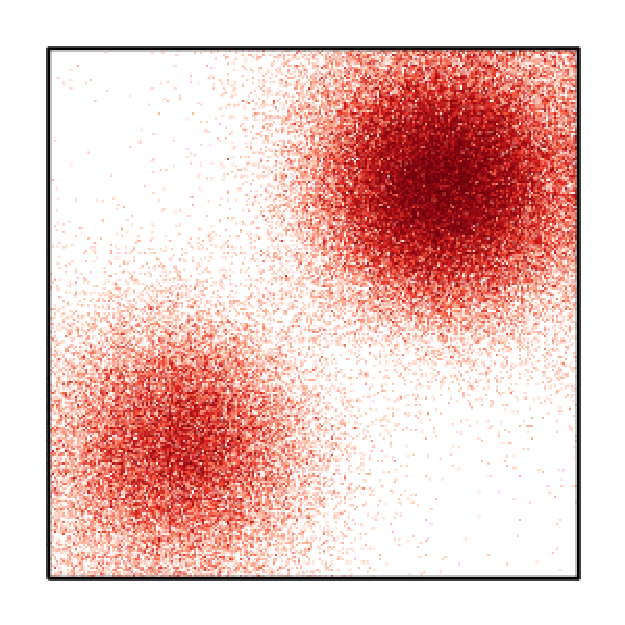
\includegraphics[width=\textwidth]{images/constraind_diffusion_rejection/synthetic_data/synthetic_hypercube_2d_rejection.pdf}
		\caption{Metropolis model}
		\label{fig:synthetic_hypercube_rejection}
	\end{subfigure}
	\hfill
	\begin{subfigure}{.195\textwidth}
		\centering
		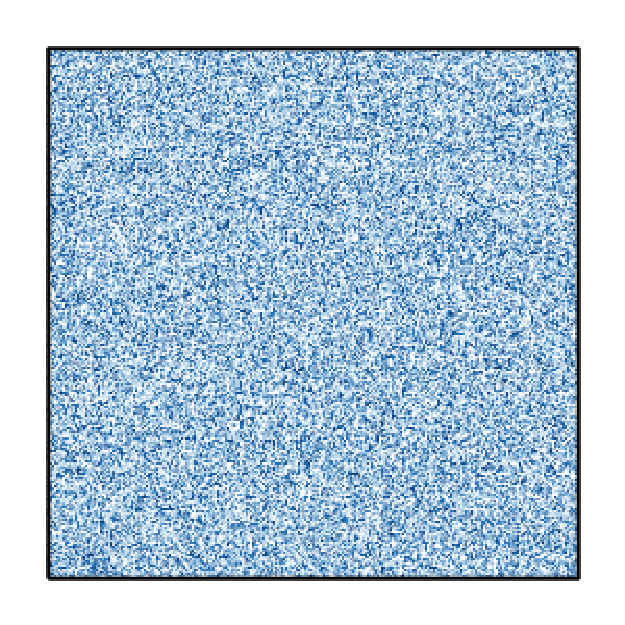
\includegraphics[width=\textwidth]{images/constraind_diffusion_rejection/synthetic_data/synthetic_hypercube_2d_uniform.pdf}
		\caption{Uniform}
		\label{fig:synthetic_hypercube_uniform}
	\end{subfigure}
	\caption{Qualitiative comparison of samples from the data distribution, our Metropolis model, a Reflected model and the uniform distribution for a synthetic bimodal distribution on \([-1, 1]^2\).}
	\label{fig:synthetic_hypercube}
\end{figure*}

\begin{figure*}[t]
	\label{fig:synthetic_dirichlet}
	\centering
	\begin{subfigure}{.195\textwidth}
		\centering
		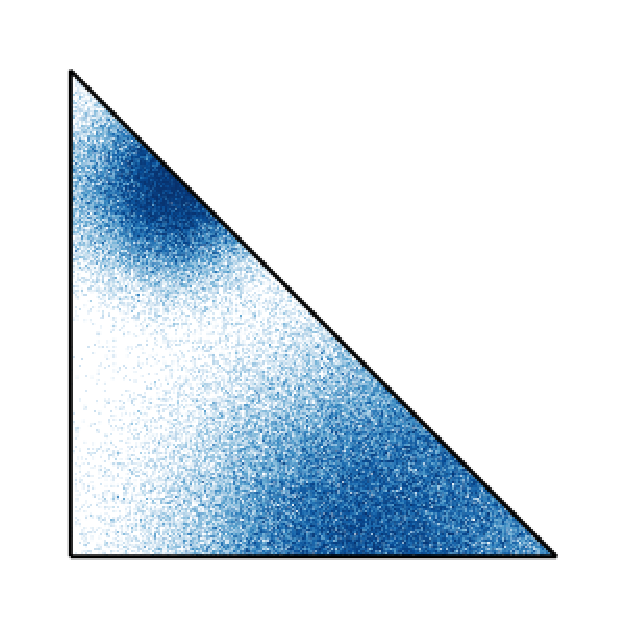
\includegraphics[width=\textwidth]{images/constraind_diffusion_rejection/synthetic_data/synthetic_dirichlet_2d_data.pdf}
		\caption{Data distribution}
		\label{fig:synthetic_simplex_data}
	\end{subfigure}
	\hfill
	\begin{subfigure}{.195\textwidth}
		\centering
		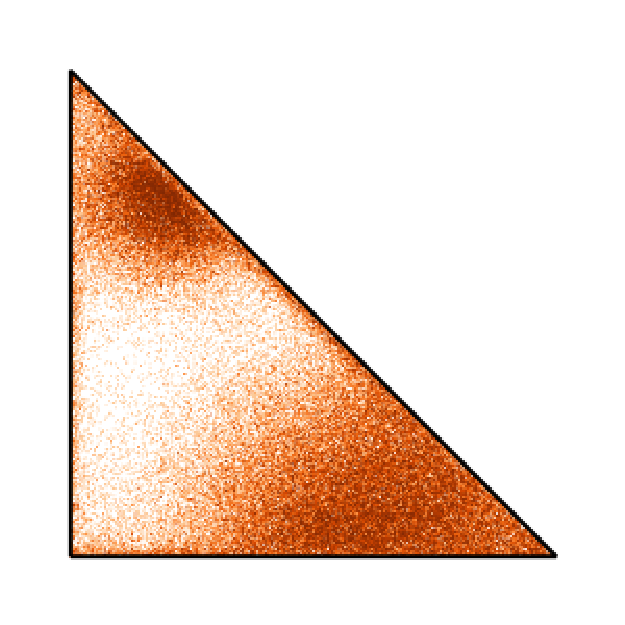
\includegraphics[width=\textwidth]{images/constraind_diffusion_rejection/synthetic_data/synthetic_dirichlet_2d_logbarrier.pdf}
		\caption{Log-barrier model}
		\label{fig:synthetic_hypercube_log-barrier}
	\end{subfigure}
	\hfill
	\begin{subfigure}{.195\textwidth}
		\centering
		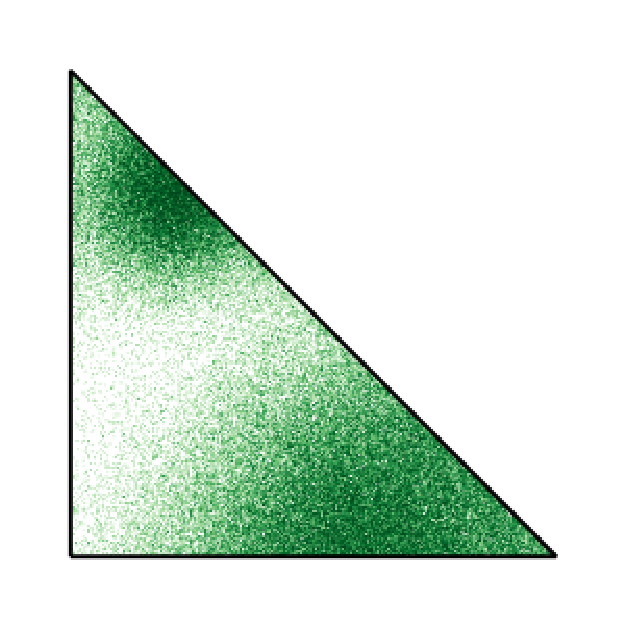
\includegraphics[width=\textwidth]{images/constraind_diffusion_rejection/synthetic_data/synthetic_dirichlet_2d_reflected.pdf}
		\caption{Reflected model}
		\label{fig:synthetic_simplex_reflected}
	\end{subfigure}
	\begin{subfigure}{.195\textwidth}
		\centering
		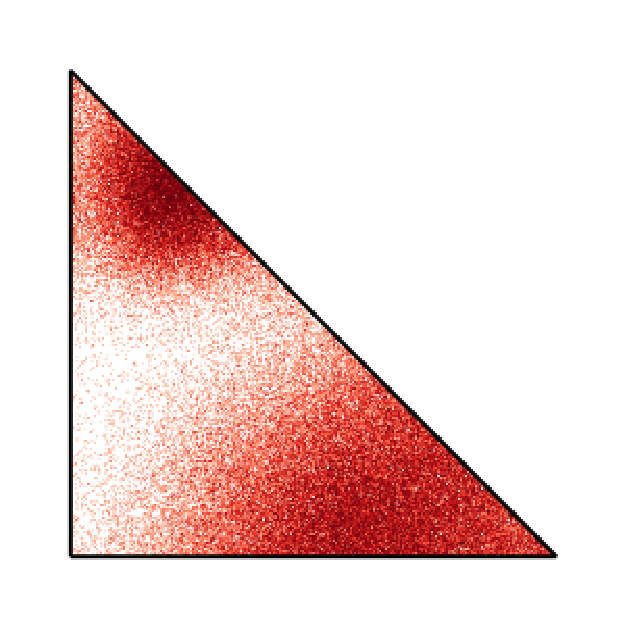
\includegraphics[width=\textwidth]{images/constraind_diffusion_rejection/synthetic_data/synthetic_dirichlet_2d_rejection.pdf}
		\caption{Metropolis model}
		\label{fig:synthetic_simplex_rejection}
	\end{subfigure}
	\hfill
	\begin{subfigure}{.195\textwidth}
		\centering
		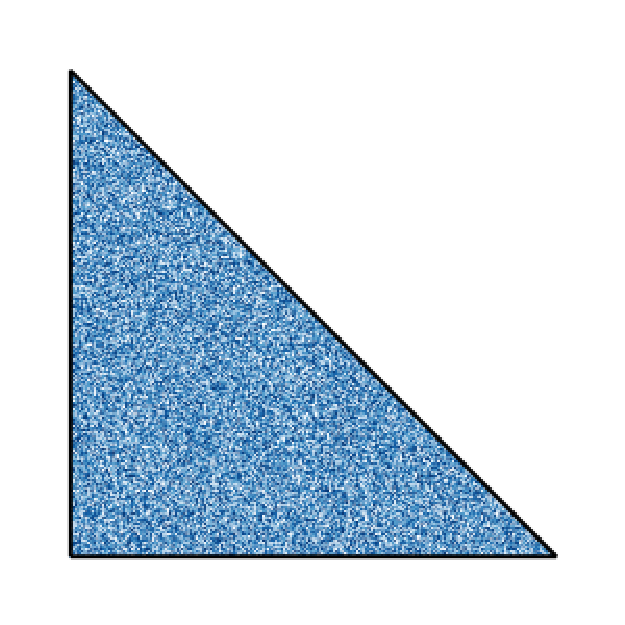
\includegraphics[width=\textwidth]{images/constraind_diffusion_rejection/synthetic_data/synthetic_dirichlet_2d_uniform.pdf}
		\caption{Uniform}
		\label{fig:synthetic_simplex_uniform}
	\end{subfigure}
	\caption{Qualitiative comparison of samples from the data distribution, our Metropolis model, a Reflected model and the uniform distribution for a synthetic bimodal distribution on \(\Delta^2\).}
	\label{fig:synthetic_simplex}
\end{figure*}

% \begin{figure}[t]
% 	\begin{subfigure}{\linewidth}
% 		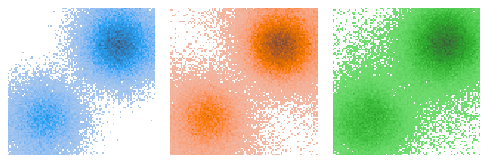
\includegraphics[width=0.8\textwidth]{images/constrained_diffusion/toy_cube.pdf}
% 		\put(-240,-10){Data}
% 		\put(-160,-10){Log-barrier}
% 		\put(-65,-10){Reflected}
% 		\caption{2D square data.}
% 	\end{subfigure}
% 	\\
% 	\begin{subfigure}{\linewidth}
% 		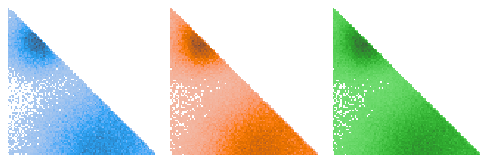
\includegraphics[width=0.8\textwidth]{images/constrained_diffusion/toy_dirichlet.pdf}
% 		\put(-240,-10){Data}
% 		\put(-160,-10){Log-barrier}
% 		\put(-65,-10){Reflected}
% 		\caption{2D square data.}
% 	\end{subfigure}
% 	\caption{
% 		Histograms of samples from the data distribution and from trained constrained diffusion models.
% 	}
% 	\label{fig:polytope_synthetic}
% \end{figure}
% \begin{table*}[t]
% 	\centering
% 	\caption{
% 		MMD metrics between samples from synthetic distributions and trained constrained and unconstrained (Euclidean) diffusion models.
% 		Means and confidence intervals are computed over 5 different runs.
% 	}
% 	\label{tab:synthetic_polytope}
% 	\begin{tabular}{cccccccc}
% 		\toprule
% 		\multirow{2}{*}{Space}      & \multirow{2}{*}{\(d\)} & \multicolumn{2}{c}{Log-barrier} & \multicolumn{2}{c}{Reflected} & \multicolumn{2}{c}{Euclidean}                                                                \\
% 		                            &                      & \textsc{MMD}                    & \(\%\in\mathcal{M}\)           & \textsc{MMD}                  & \(\%\in\mathcal{M}\) & \textsc{MMD}     & \(\%\in\mathcal{M}\) \\
% 		\midrule
% 		\multirow{3}{*}{\([-1,1]^d\)} & 2                    & \(.066 \pm{.006}\)                & 100.0                         & \(.055 \pm{.015}\)              & 100.0               & \(.062 \pm{.011}\) & 98.8                \\
% 		                            & 3                    & \(.209 \pm{.077}\)                & 100.0                         & \(.080 \pm{.004}\)              & 100.0               & \(.076 \pm{.004}\) & 98.5                \\
% 		                            & 10                   & \(.330 \pm{.004}\)                & 100.0                         & \(.313 \pm{.048}\)              & 100.0               & \(.081 \pm{.005}\) & 96.4                \\
% 		\midrule
% 		\multirow{3}{*}{\(\Delta^d\)} & 2                    & \(.050 \pm{.012}\)                & 100.0                         & \(.043 \pm{.002}\)              & 100.0               & \(.055 \pm{.013}\) & 96.4                \\
% 		                            & 3                    & \(.238 \pm{.009}\)                & 100.0                         & \(.181 \pm{.007}\)              & 100.0               & \(.068\pm{.014}\)  & 96.3                \\
% 		                            & 10                   & \(.275 \pm{.015}\)                & 100.0                         & \(.290 \pm{.009}\)              & 100.0               & \(.060	\pm{.003}\) & 92.6                \\
% 		\bottomrule
% 	\end{tabular}
% \end{table*}
\begin{table*}[t]
	\caption{
		Maximum mean discrepancy (MMD) (\(\downarrow\)) of a held-out test set from a synthetic bimodal distribution over convex subsets of \(\R^d\) bounded by the hypercube \([-1,1]^d\) and unit simplex \(\Delta^d\).
		Means and standard deviations are computed over 3 different runs.
	}
	\label{tab:synthetic_polytope_mmd}
	\vspace{1em}
	\centering

	\begin{tabular}{ccr@{}lr@{}lr@{}lr@{}lc}
		\toprule
		\multirow{2}{*}{Space} & \multirow{2}{*}{\(d\)} & \multicolumn{2}{c}{\scshape Log-Barrier}                & \multicolumn{2}{c}{\scshape Reflected}                  & \multicolumn{2}{c}{\scshape Metropolis}                 & \multicolumn{3}{c}{\scshape Euclidean}                                                                                                     \\
		                       &                      & \multicolumn{2}{c}{\textsc{MMD}\emph{(hours)}} & \multicolumn{2}{c}{\textsc{MMD}\emph{(hours)}} & \multicolumn{2}{c}{\textsc{MMD}\emph{(hours)}} & \multicolumn{2}{c}{\textsc{MMD}\emph{(hours)}} & \(\%\in\mathcal{M}\)                                                               \\
		\midrule
		\multirow{3}{*}{\([-1,1]^d\)}
		                       & 2                    & \(.066_{\pm{.006}}\)                             & \emph{(0.00)}                                  & \(.055_{\pm{.015}}\)                             & \emph{(8.95)}                                  & \({.029_{\pm{.002}}}\) & \emph{(0.72)} & \(.062_{\pm{.011}}\) & \emph{(0.00)} & 98.8 \\
		                       & 3                    & \(.209_{\pm{.077}}\)                             & \emph{(0.00)}                                  & \(.080_{\pm{.004}}\)                             & \emph{(8.97)}                                  & \({.047_{\pm{.006}}}\) & \emph{(0.71)} & \(.076_{\pm{.004}}\) & \emph{(0.00)} & 98.5 \\
		                       & 10                   & \(.330_{\pm{.004}}\)                             & \emph{(0.00)}                                  & \(.313_{\pm{.048}}\)                             & \emph{(10.15)}                                 & \({.226_{\pm{.006}}}\) & \emph{(0.90)} & \(.081_{\pm{.005}}\) & \emph{(0.00)} & 96.4 \\
		                    %    & 50                   & -                                              & -                                              & -                                              & -                                              & \({.???_{\pm{.???}}}\) & \emph{(?.??)} & \(.???_{\pm{.???}}\) & \emph{(?.??)} & ??.? \\
		                    %    & 100                  & -                                              & -                                              & -                                              & -                                              & \({.???_{\pm{.???}}}\) & \emph{(?.??)} & \(.???_{\pm{.???}}\) & \emph{(?.??)} & ??.? \\
		\midrule
		\multirow{3}{*}{\(\Delta^d\)}
		                       & 2                    & \(.050_{\pm{.012}}\)                             & \emph{(0.00)}                                  & \(.043_{\pm{.002}}\)                             & \emph{(9.17)}                                  & \({.032_{\pm{.007}}}\) & \emph{(0.82)} & \(.055_{\pm{.013}}\) & \emph{(0.00)} & 96.4 \\
		                       & 3                    & \(.238_{\pm{.009}}\)                             & \emph{(0.00)}                                  & \(.181_{\pm{.007}}\)                             & \emph{(9.43)}                                  & \({.121_{\pm{.010}}}\) & \emph{(0.78)} & \(.068_{\pm{.014}}\) & \emph{(0.00)} & 96.3 \\
		                       & 10                   & \(.275_{\pm{.015}}\)                             & \emph{(0.00)}                                  & \(.290_{\pm{.009}}\)                             & \emph{(10.53)}                                 & \({.260_{\pm{.003}}}\) & \emph{(0.97)} & \(.060_{\pm{.003}}\) & \emph{(0.00)} & 92.6 \\
		                    %    & 50                   & -                                              & -                                              & -                                              & -                                              & \({.???_{\pm{.???}}}\) & \emph{(?.??)} & \(.???_{\pm{.???}}\) & \emph{(?.??)} & ??.? \\
		                    %    & 100                  & -                                              & -                                              & -                                              & -                                              & \({.???_{\pm{.???}}}\) & \emph{(?.??)} & \(.???_{\pm{.???}}\) & \emph{(?.??)} & ??.? \\
		\bottomrule
	\end{tabular}
\end{table*}

\subsection{Modelling robotic arms under force and velocity constraints}
\label{sec:exp_constrained_robot}
Next we move on to a modelling problem motivated by robotics.

Accurately determining and controlling the movement and exerted forces of robotic platforms is a fundamental problem in many real-world robotics applications.
A kinetostatic descriptor that is commonly used to quantify the ability of a robotic arm to move and apply forces along certain dimensions is the so-called manipulability ellipsoid \(E\in\mathbb{R}^d\) \parencite{yoshikawa1985manipulability} which is naturally described as a symmetric positive definite (SPD) matrix \(\mathrm{M} \in\mathbb{R}^{d\times d}\) \parencite{jaquier2021geometry}.
The manifold of such \(d\times d\) SPD matrices, denoted as \(S_{++}^d\), is defined as the set of matrices \( \{ x^\top \mathrm{M} x \geq 0 , \ x\in \mathbb{R}^d : \mathrm{M} \in \R^{d \times d} \} \).

In many practical settings, it may be desirable to constrain the volume of \(E\) to retain flexibility or limit the magnitude of an exerted force, which can be expressed as an upper bound on the trace of \(\mathrm{M}\), i.e.\ as the inequality constraint \(\sum_{i=1}^d \mathrm{M}_{ii} < C\) with \(C >0\).
Constraining the rest of the entries of the matrix to ensure it is SPD is non-trivial.

Alternatively, we can parameterise the SPD matrices via their Cholesky decomposition.
Each SPD matrix has a unique decomposition of the form \(\mathrm{M} = \mathrm{L} \mathrm{L}^\top\), where \( \mathrm{L}\) is a lower triangular matrix with strictly positive diagonal \parencite[p.143]{golub2013matrix}.
Constraining the entries of this matrix simply requires ensuring the diagonal is positive.
The trace of the SPD matrix is given by \(\mathrm{Tr}(\mathrm{M}) = \mathrm{Tr}(\mathrm{L} \mathrm{L}^\top) = \sum_{ij}\mathrm{L}_{ij}^2\), and results in the constraint on the entries of \(\mathrm{L}\) to live in a ball of radius \(C\).
We additionally model the two-dimensional position of the arm.

In summary, the space over which we parameterise the diffusion models is defined as \(\{ \mathrm{L} \in \R^{d(d+1)/2} : \mathrm{L}_{i,i} > 0, \sum_{i,j} \mathrm{L}_{i,j}^2 < C \} \times \R^2\).
Under the Euclidean metric, we can apply all of the log-barrier, reflected, and metropolised approaches.
The positive diagonal (linear) constraint is handled similarly to the polytope setting.
The reflection on the ball boundary is defined and illustrated on \cref{fig:reflection_diagrams_lin,fig:reflection_diagrams_sph}.

\begin{figure*}[t]
	\centering
	\begin{subfigure}{0.195\textwidth}
		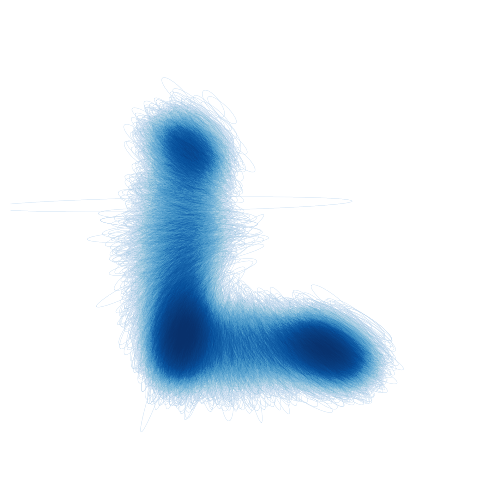
\includegraphics[width=\textwidth]{images/constrained_diffusion/spd_l_data.png}
		\caption{Data distribution}
	\end{subfigure}
	\hfill
	\begin{subfigure}{0.195\textwidth}
		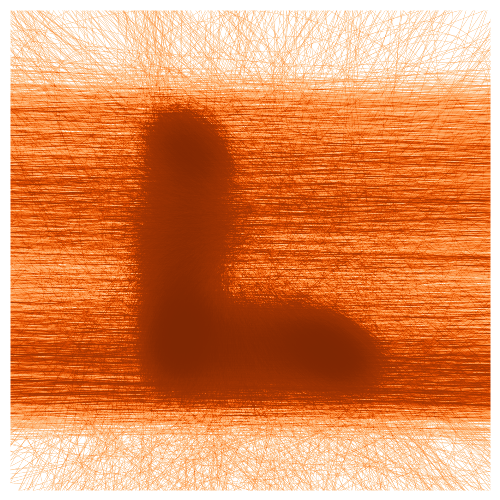
\includegraphics[width=\textwidth]{images/constrained_diffusion/spd_l_logbarrier.png}
		\caption{Log-barrier model}
	\end{subfigure}
	\hfill
	\begin{subfigure}{0.195\textwidth}
		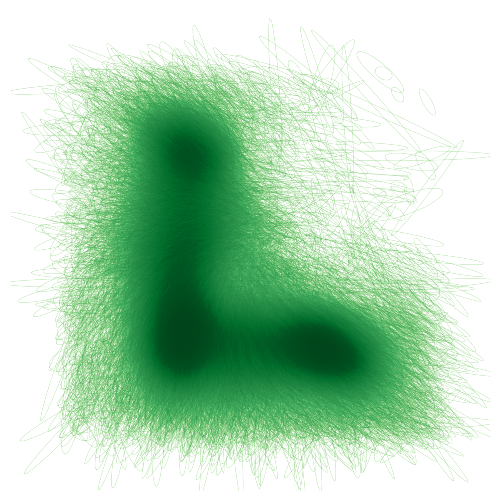
\includegraphics[width=\textwidth]{images/constraind_diffusion_rejection/spd_main_reflected.png}
		\caption{Reflected model}
	\end{subfigure}
	\hfill
	\begin{subfigure}{0.195\textwidth}
		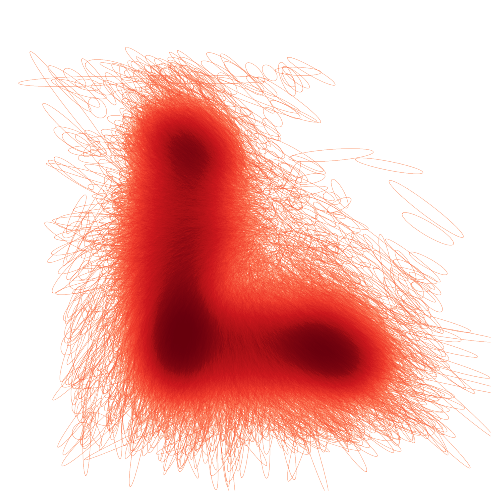
\includegraphics[width=\textwidth]{images/constraind_diffusion_rejection/spd_main_rejection.png}
		\caption{Metropolis model}
	\end{subfigure}
	\hfill
	\begin{subfigure}{0.195\textwidth}
		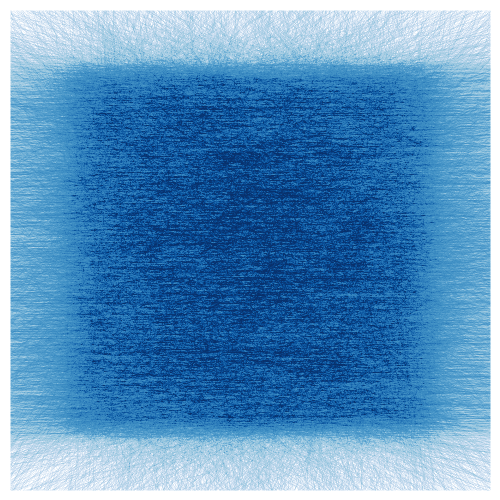
\includegraphics[width=\textwidth]{images/constrained_diffusion/spd_l_uniform.png}
		\caption{Uniform}
	\end{subfigure}
	\caption{Samples in \(S_{++}^2\times\mathbb{R}^2\) from (a) the data distribution, (b) our log-barrier diffusion model, (c) our reflected diffusion model and (d) the uniform distribution.
		Each sample is visualised as the manipulability ellipsoid encoded by the SPD matrix \(M\in S_{++}^2\) placed at the corresponding location in \(\mathbb{R}^2\).
		Additional results and full correlation plots are postponed to~\Cref{sec:app_spd_exp}.
	}
	\label{fig:spd_data}
\end{figure*}

Using this framework, we model the datasets presented in \cite{jaquier2021geometry} (see \cref{sec:robotic_arm} for full experimental details).
The joint distribution over the SPD matrices (represented as ellipsoids) and their positions is presented in~\cref{fig:spd_data}.
We qualitatively observe that the reflected method is able to fit the joint data distribution.
In \cref{tab:robotics_mmd_results} we observe that the reflected and metropolis results significantly outperfrom the log-barrier method, and the metropolois method outperforms the reflected approch slightly.

\begin{table}[h]
	\caption{
		Maximum mean discrepancy (MMD) (\(\downarrow\)) between samples from the trained model and a held-out test set from the robotics data.
		Means and standard deviations are computed over 3 different runs.
	}
	\label{tab:robotics_mmd_results}
	\centering

	\begin{tabular}{rccc}
		\toprule
		& {\scshape Log-Barrier}                & {\scshape Reflected}                  & {\scshape Metropolis} \\
		\midrule
		\scshape MMD &\(0.247_{\pm 0.03}\) & \(0.161_{\pm 0.02}\) & \( 0.152_{\pm 0.03}\) \\
		\bottomrule
	\end{tabular}
\end{table}

\subsection{Modelling proteins under loop constraints}
\label{sec:exp_constrained_protein}

Modelling the conformational ensembles of proteins is an important task in the field of molecular biology, particularly in the context of bioengineering and drug discovery.

As the deviation of chemical bond lengths and angles from their theoretical average is generally negligible, the problem of modelling the three-dimensional structure of this polypeptide chain is often reframed in the space of the internal torsion angles \(\Phi\) and \(\Psi\) (see~\cref{fig:peptide_chain} for an illustration), which can be modelled on a \((2N-2)\)-dimensional torus \(\mathbb{T}^{2N-2}\).
\begin{figure}[t]
	\centering
	\begin{subfigure}{0.45\textwidth}
		\centering
		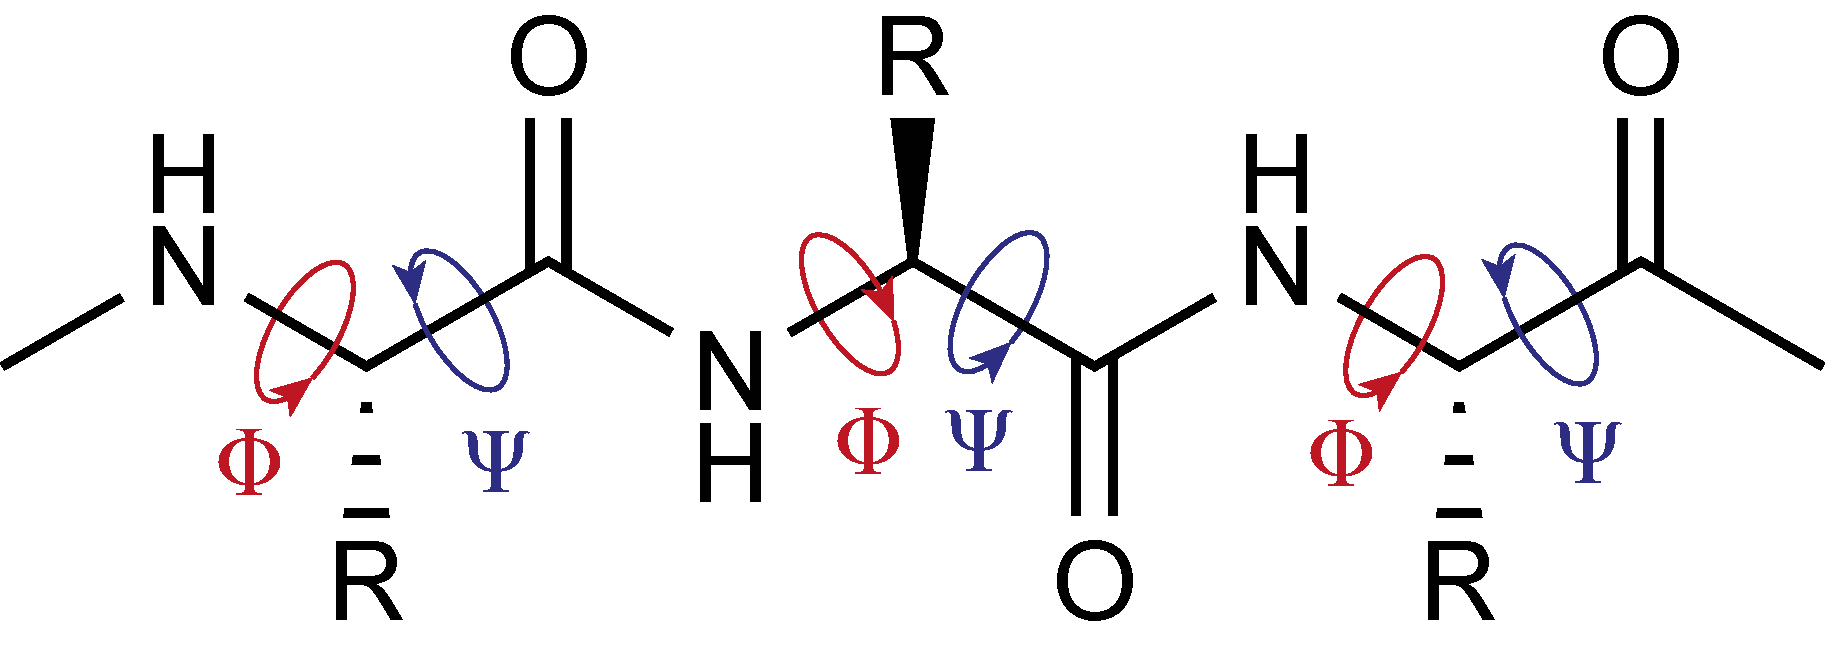
\includegraphics[width=\linewidth]{images/constrained_diffusion/peptide_chain.pdf}
		\caption{A commonly-used approximate parameterisation of backbone geometry only considers the \(C_\alpha\) torsion angles \(\Phi\) and \(\Psi\).}
		\label{fig:peptide_chain}
	\end{subfigure}
	\hspace{0.5cm}
	\begin{subfigure}{0.45\textwidth}
		\centering
		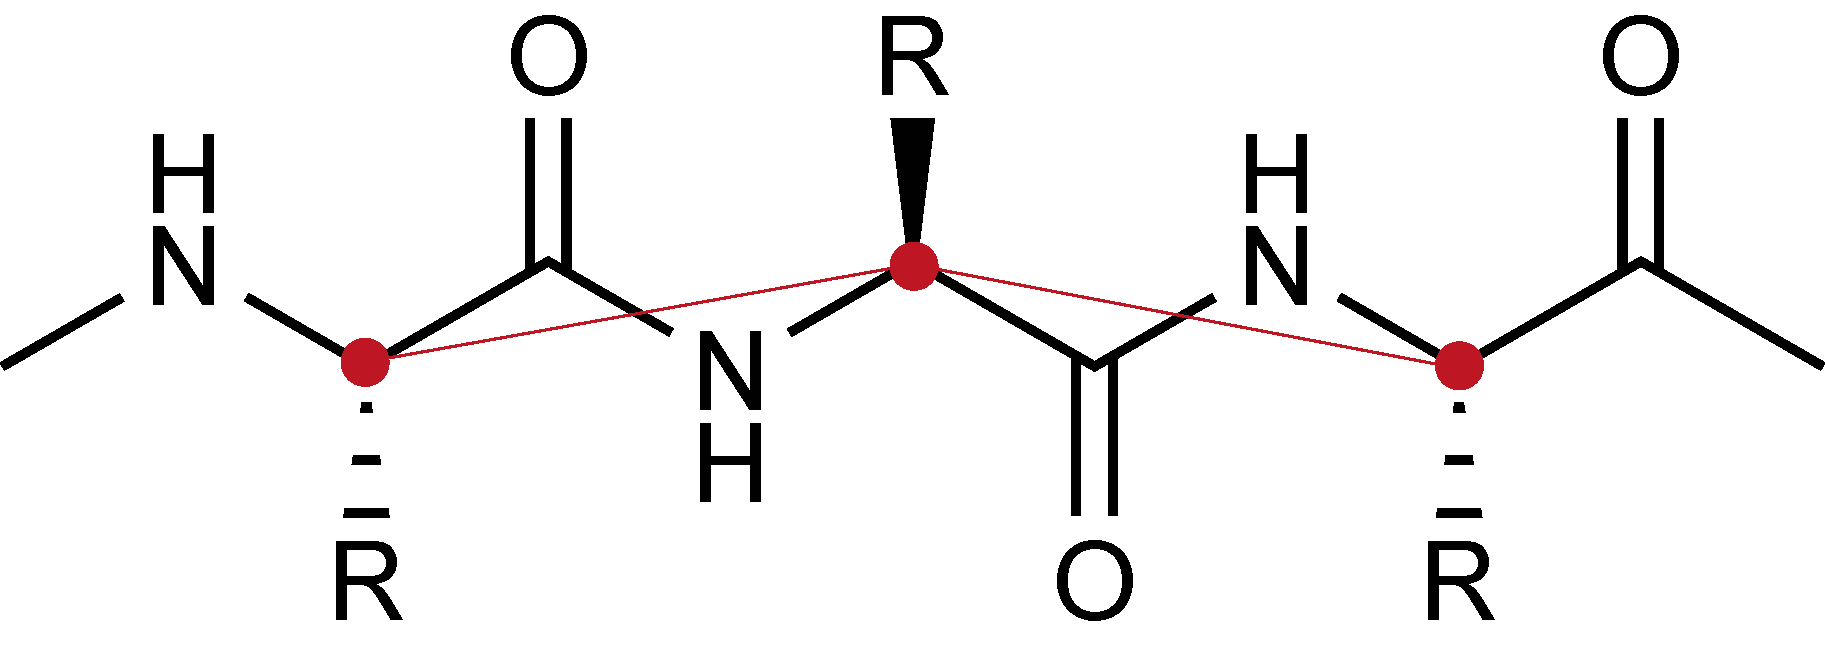
\includegraphics[width=\linewidth]{images/constrained_diffusion/ca_trace.pdf}
		\caption{As peptide bond orientations can be inferred relatively reliably, researchers often only model the \(C_\alpha\) traces.}
		\label{fig:peptide_trace}
	\end{subfigure}
	\caption{Standard approaches to modelling the conformations of polypeptide backbones.}
	\label{fig:peptide}
\end{figure}

In many data-scarce practical settings such as antibody or enzyme design, it is often unnecessary or even undesirable to model the structure of an entire protein however, as researchers are primarily interested in specific functional sites with distinct biochemical properties.
However, generating conformational ensembles for such substructural elements necessitates positional constraints on their endpoints to ensure that they can be accommodated by the remaining scaffold.

\begin{figure}[t]
	\centering
	\vspace{-0.5cm}
	\begin{subfigure}[t]{0.45\textwidth}
		\centering
		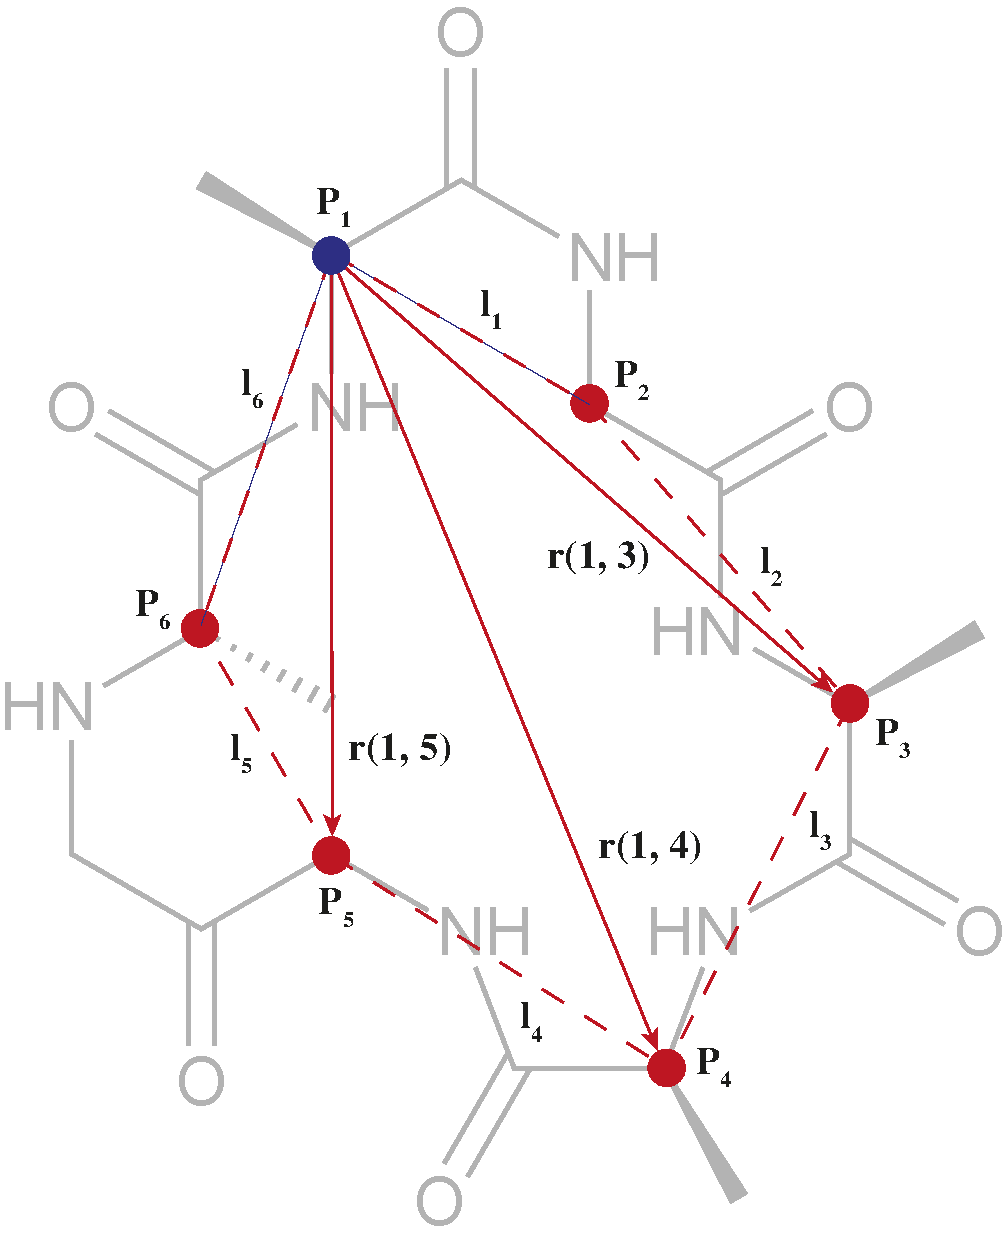
\includegraphics[height=4cm]{images/constrained_diffusion/cyclic_peptide.pdf}
		\caption{An illustrative diagram of the parameterisation used for the conformational modelling of the \(C_\alpha\) trace of a cyclic peptide, introduced in \cite{han2006inverse}.}
		\label{fig:cyclic_peptide_main}
	\end{subfigure}
	\hfill
	\begin{subfigure}[t]{0.45\textwidth}
		\centering
		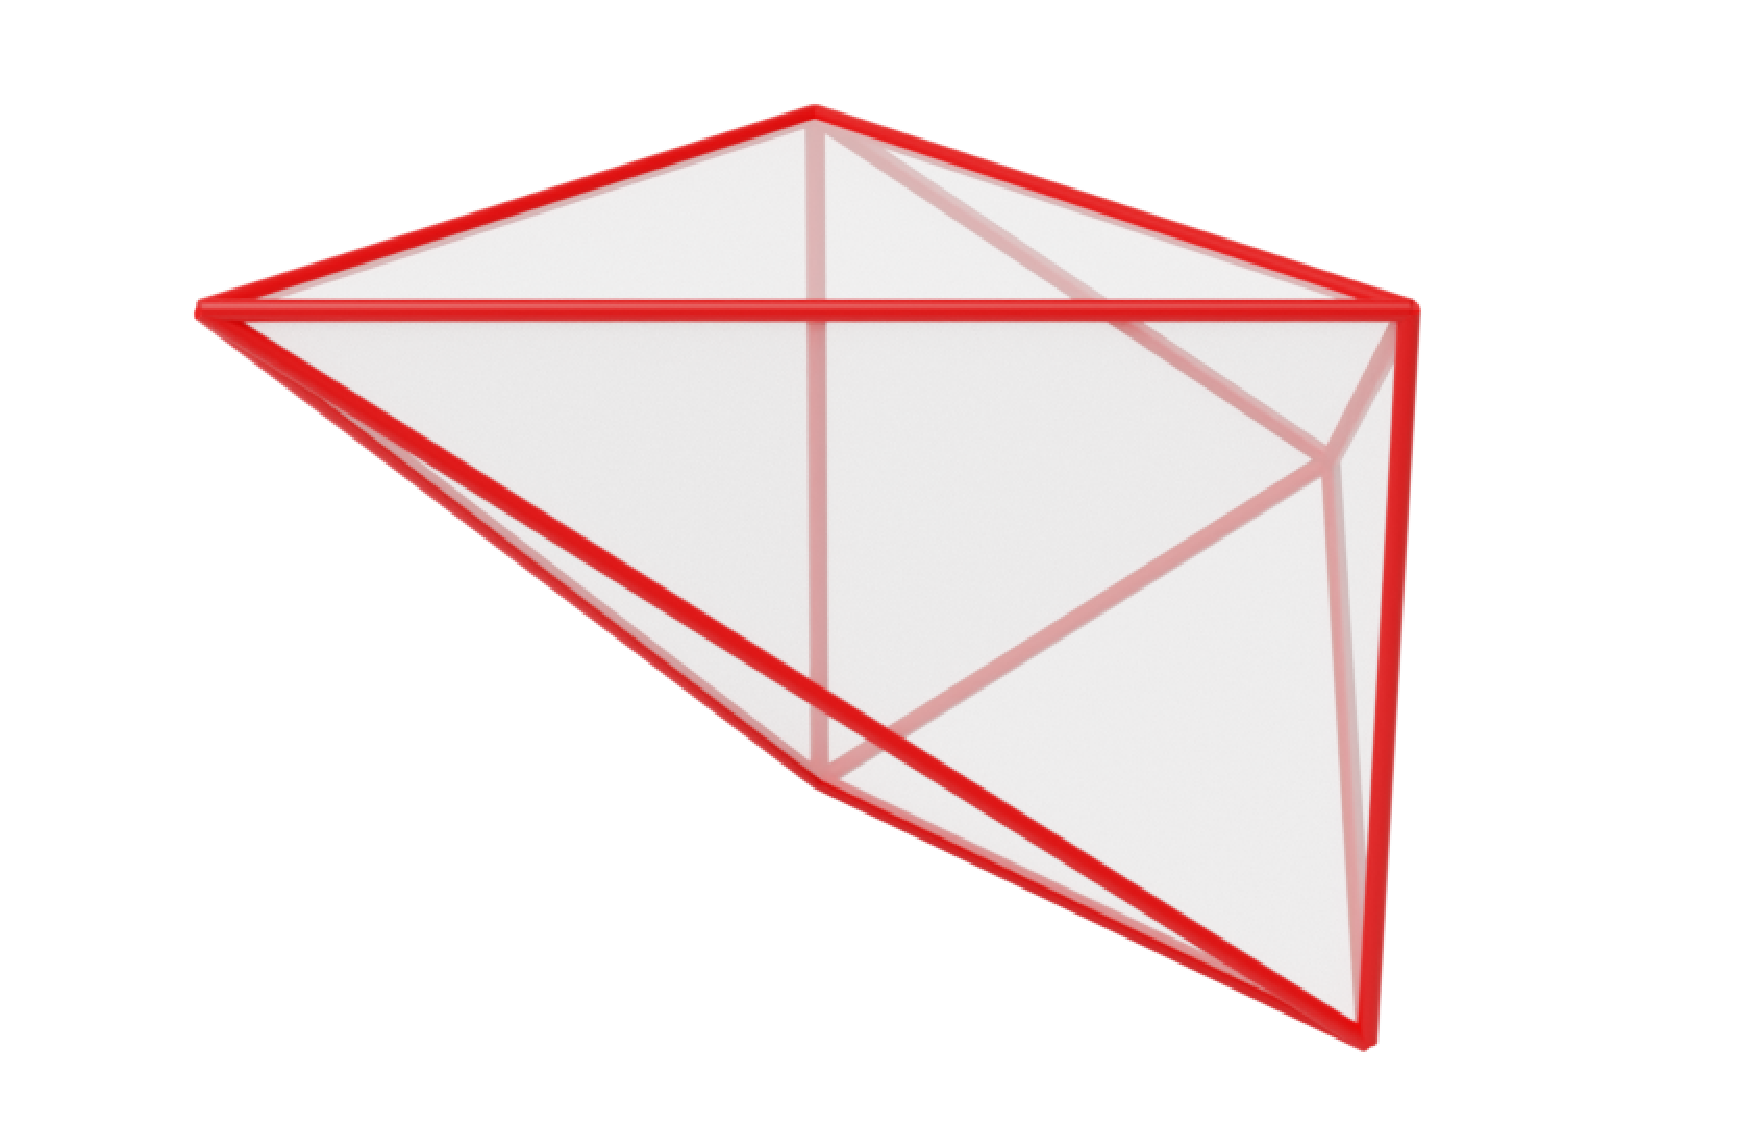
\includegraphics[height=4cm]{images/constrained_diffusion/hull.pdf}
		\caption{The convex polytope constraining the diagonals of the triangles for the given bond lengths in the illustrated molecule.
			The total design space is the product of this polytope with the 4D flat torus.
		}
		\label{fig:6s_random_walk_main}
	\end{subfigure}
	\caption{Illustrations of the parametrisation used to model distribution of polypeptide backbone conformations under anchor point distance constraints as the product of a convex polytope \(\mathbb{P}\) and torus \(\mathbb{T}\): \(\mathbb{P}^{3} \times \mathbb{T}^{4}\).}
	\label{fig:han_and_rudolph_main}
\end{figure}

This problem can be reformulated as modelling a spatial chain with spherical joints and fixed end points.
Following the framework outlined in \textcite{han2006inverse}, we parametrise the conformations of such chains with \(d\) fixed-length links and arbitrary end-point constraints as the product of a convex polytope \(\mathbb{P}\) and torus \(\mathbb{T}\): \(\mathbb{P}^{(d-2)} \times \mathbb{T}^{(d-1)}\).
The essential idea in this parameterisation is to fix one end point as an ``anchor'' and model the chain as the series of triangles formed by the anchor and each pair of adjacent joints in the chain.
A point in the polytope corresponds to the lengths of the diagonals of these triangles, and a point in the torus to the angles between each subsequent triangle.
See~\Cref{fig:han_and_rudolph_main} for an illustration and \Cref{sec:protein_param} for a full description.
Using this framework, we model the conformational landscape of the cyclic peptide \textsc{c-AAGAGG}, consisting of a circular polypeptide chain with coinciding endpoints.
We generate \(10^6\) backbone conformations using tools from molecular dynamics \parencite{eastman2017openmm, hornak2006comparison} and divide them into training and evaluation datasets, (see~\Cref{sec:protein_data} for full experimental details).
Drawing on the definition above, the space on which we effectively parameterise our constrained diffusion models for a circular polypeptide chain of length \(d=6\) is given by the product manifold \(\mathbb{P}^3 \times \mathbb{T}^4\).

% \subsubsection{Modelling the problem}

\begin{figure*}[tb]
	\centering
	\begin{subfigure}{0.19\textwidth}
		\centering
		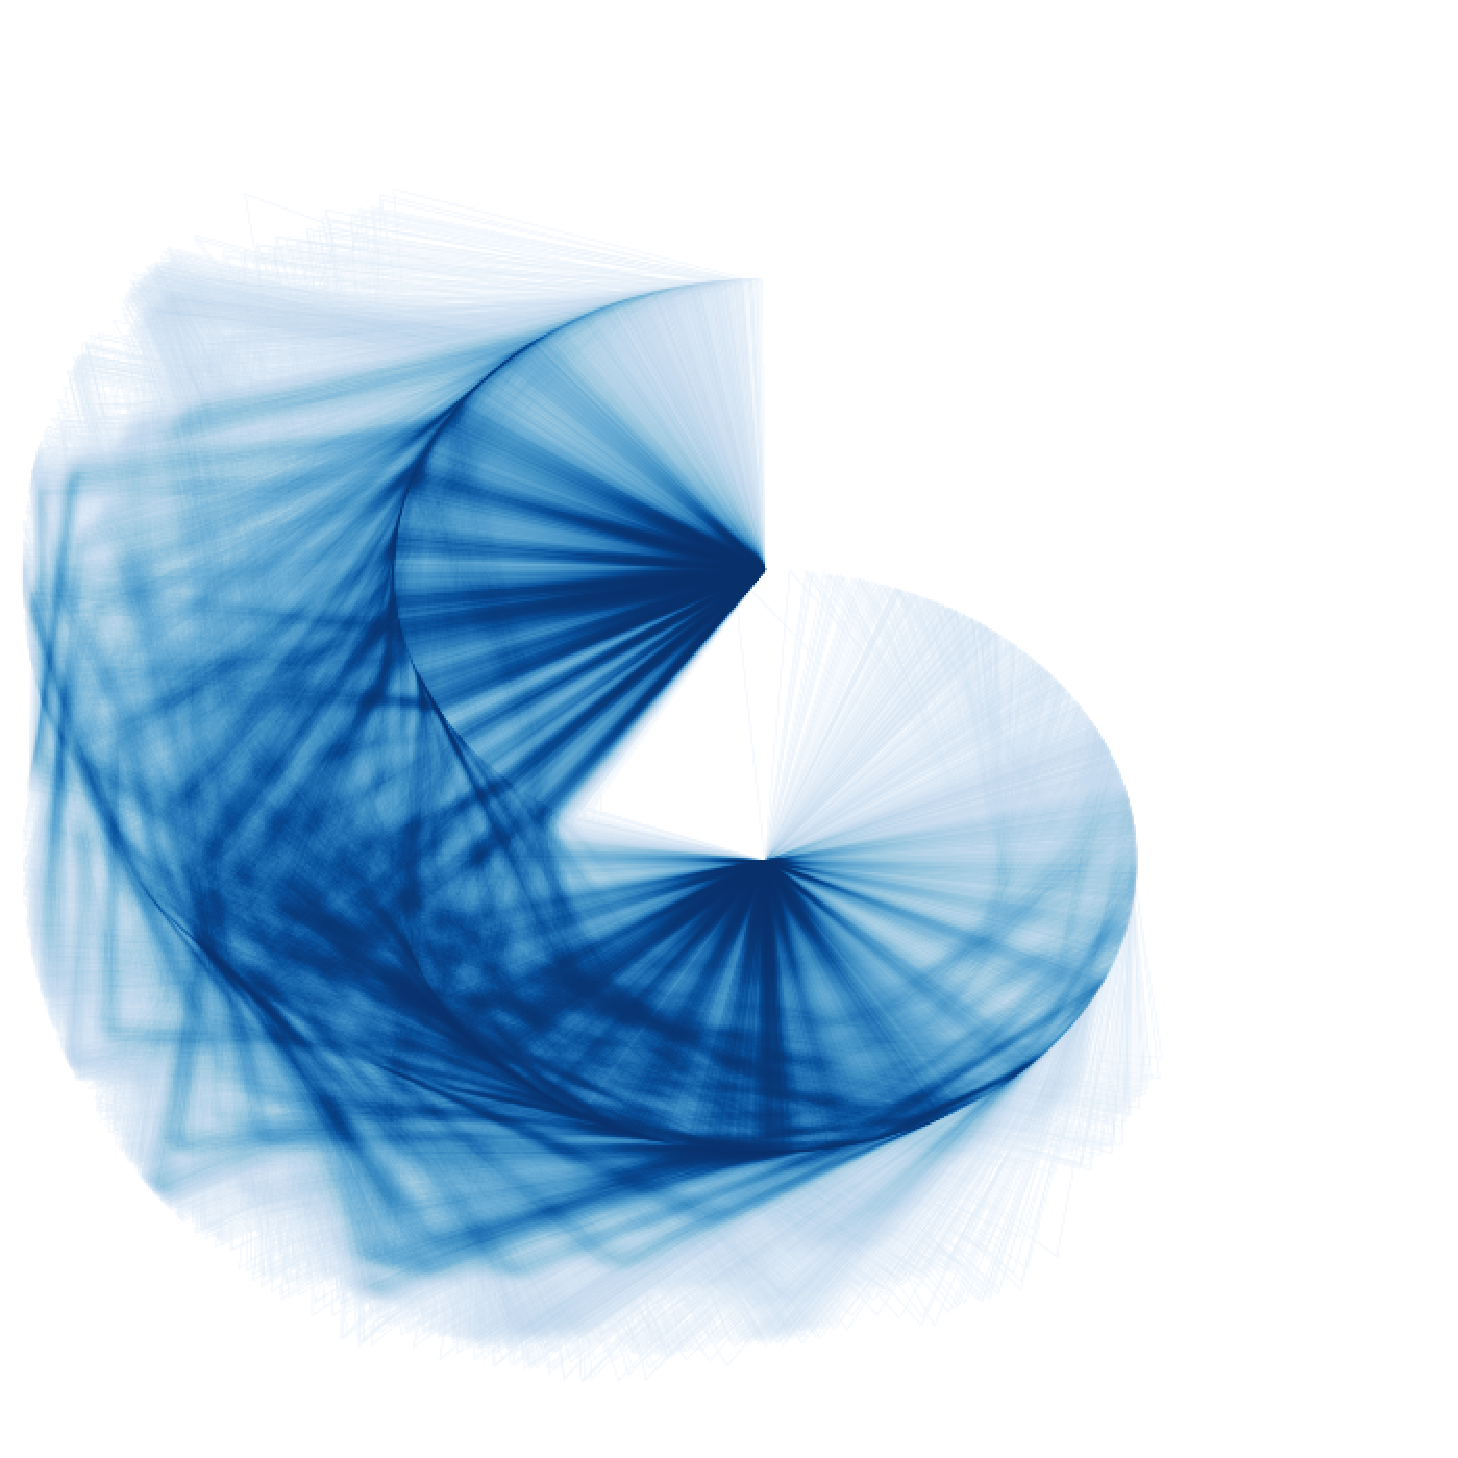
\includegraphics[width=\linewidth]{images/constrained_diffusion/loop_data_dist_2d.pdf}
		\caption{Data}
		\label{fig:loop_plot_smoothened}
	\end{subfigure}
	\hfill
	\begin{subfigure}{0.1919\textwidth}
		\centering
		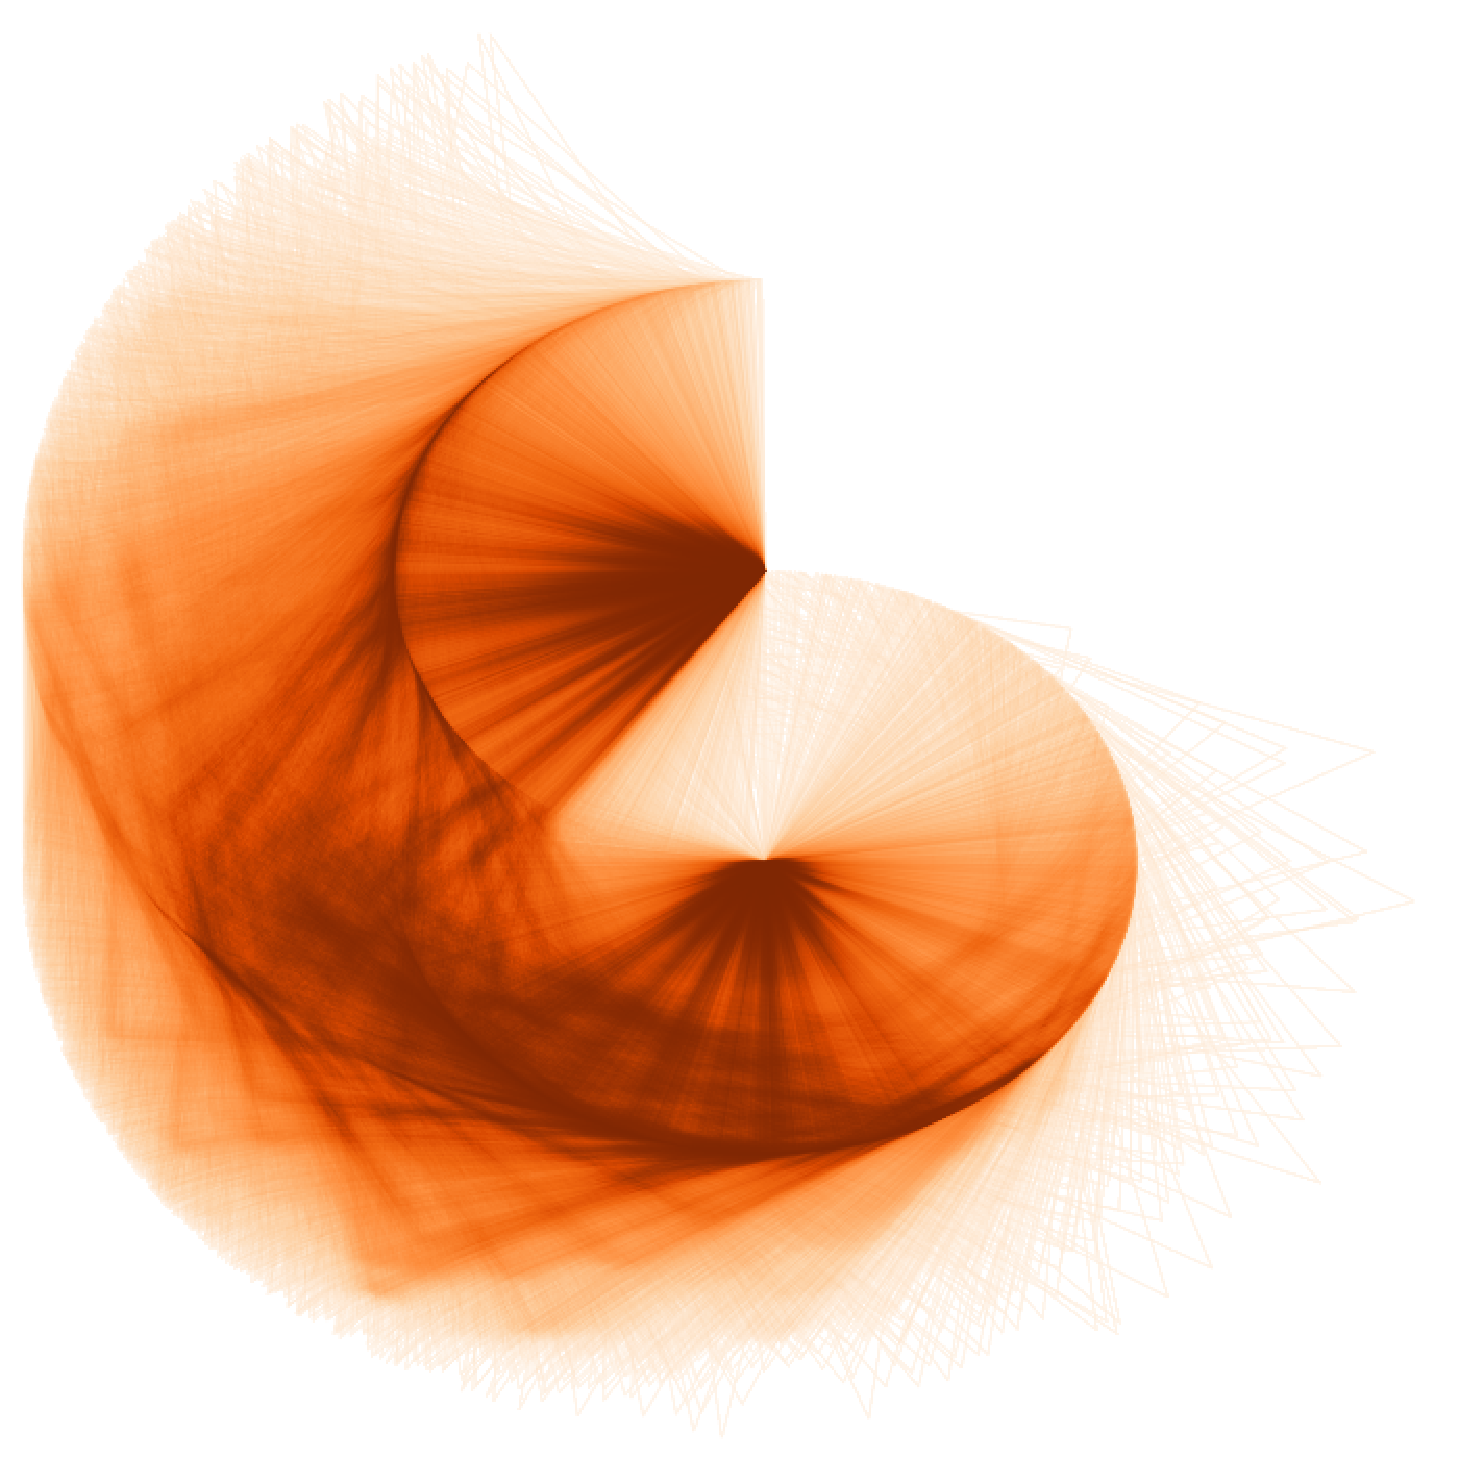
\includegraphics[width=\linewidth]{images/constrained_diffusion/loop_logbarrier_dist_2d.pdf}
		\caption{Log-barrier}
		\label{fig:loop_plot_logbarrier}
	\end{subfigure}
	\hfill
	\begin{subfigure}{0.19\textwidth}
		\centering
		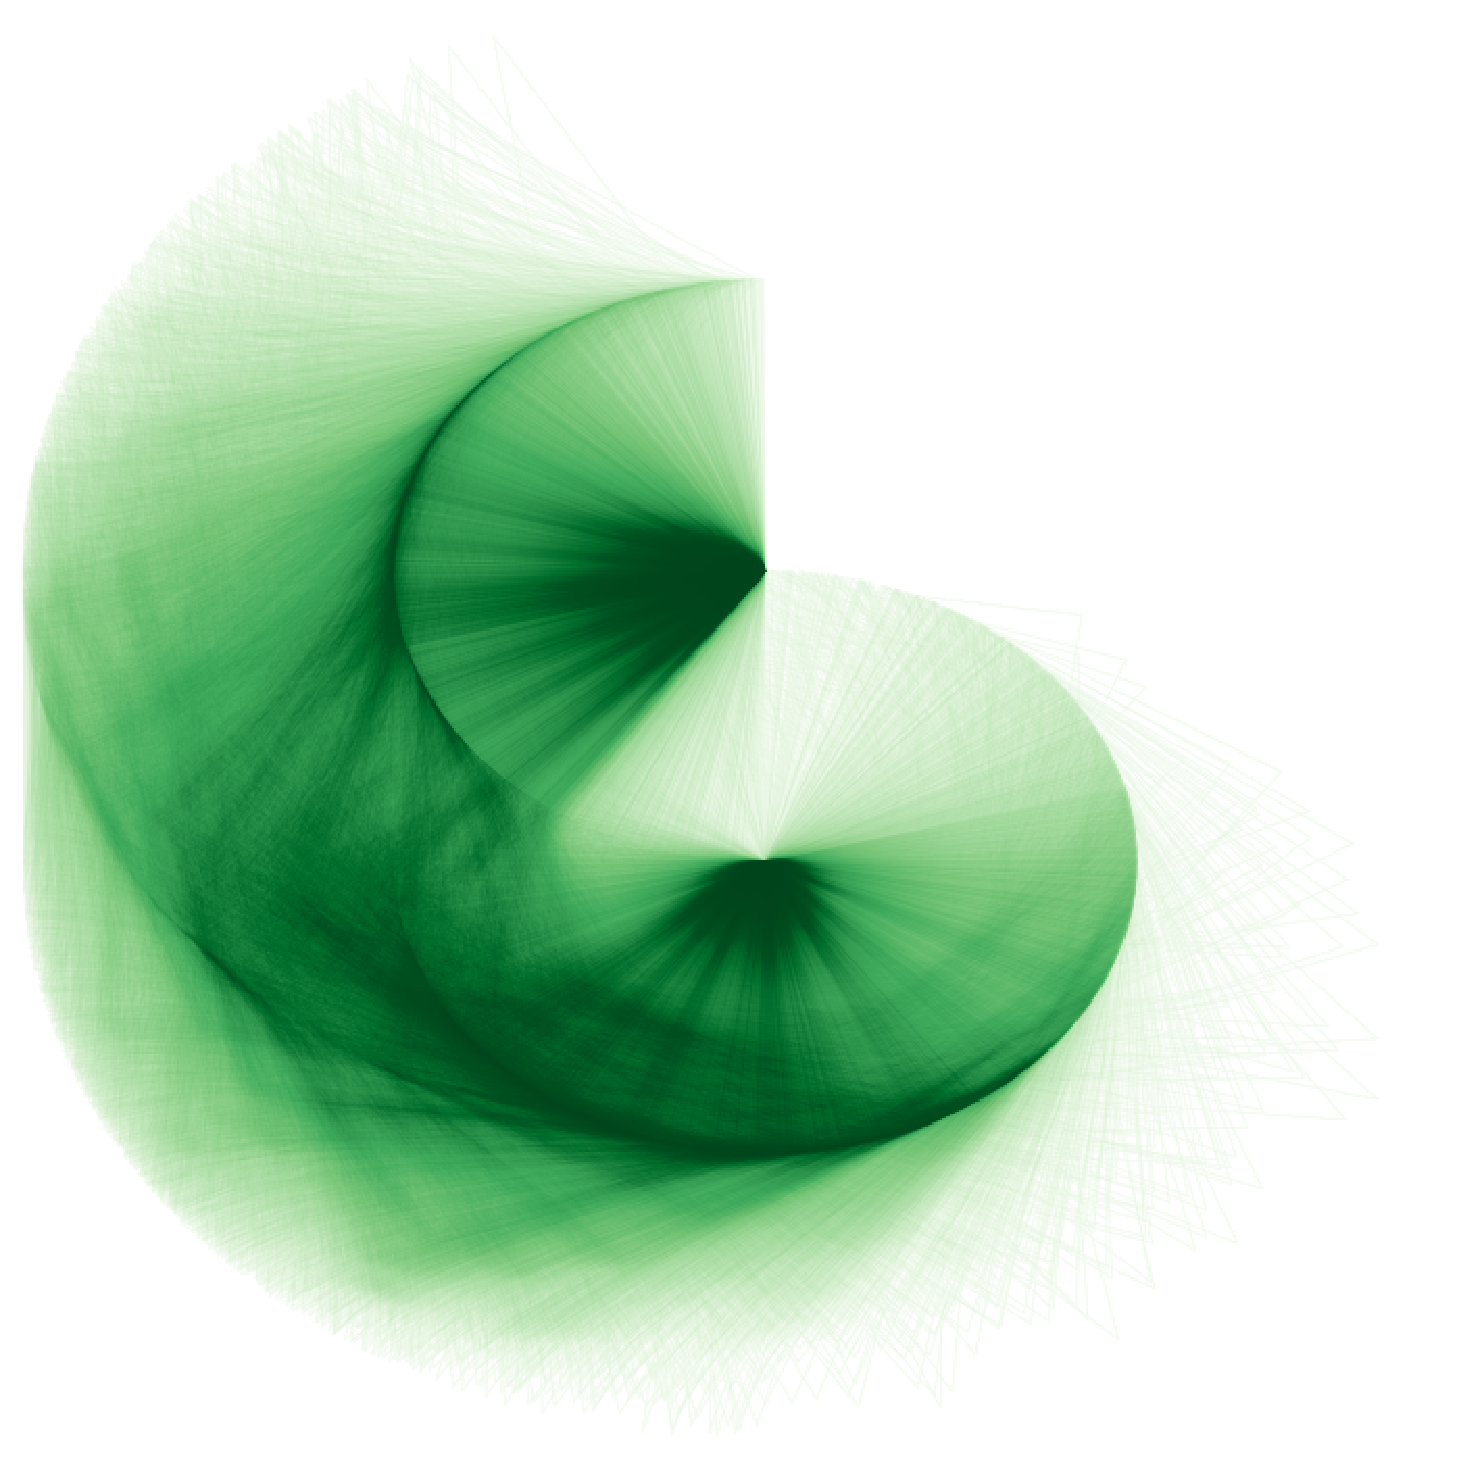
\includegraphics[width=\linewidth]{images/constrained_diffusion/loop_reflected_dist_2d.pdf}
		\caption{Reflected}
		\label{fig:loop_plot_sampled}
	\end{subfigure}
	\hfill
	\begin{subfigure}{0.19\textwidth}
		\centering
		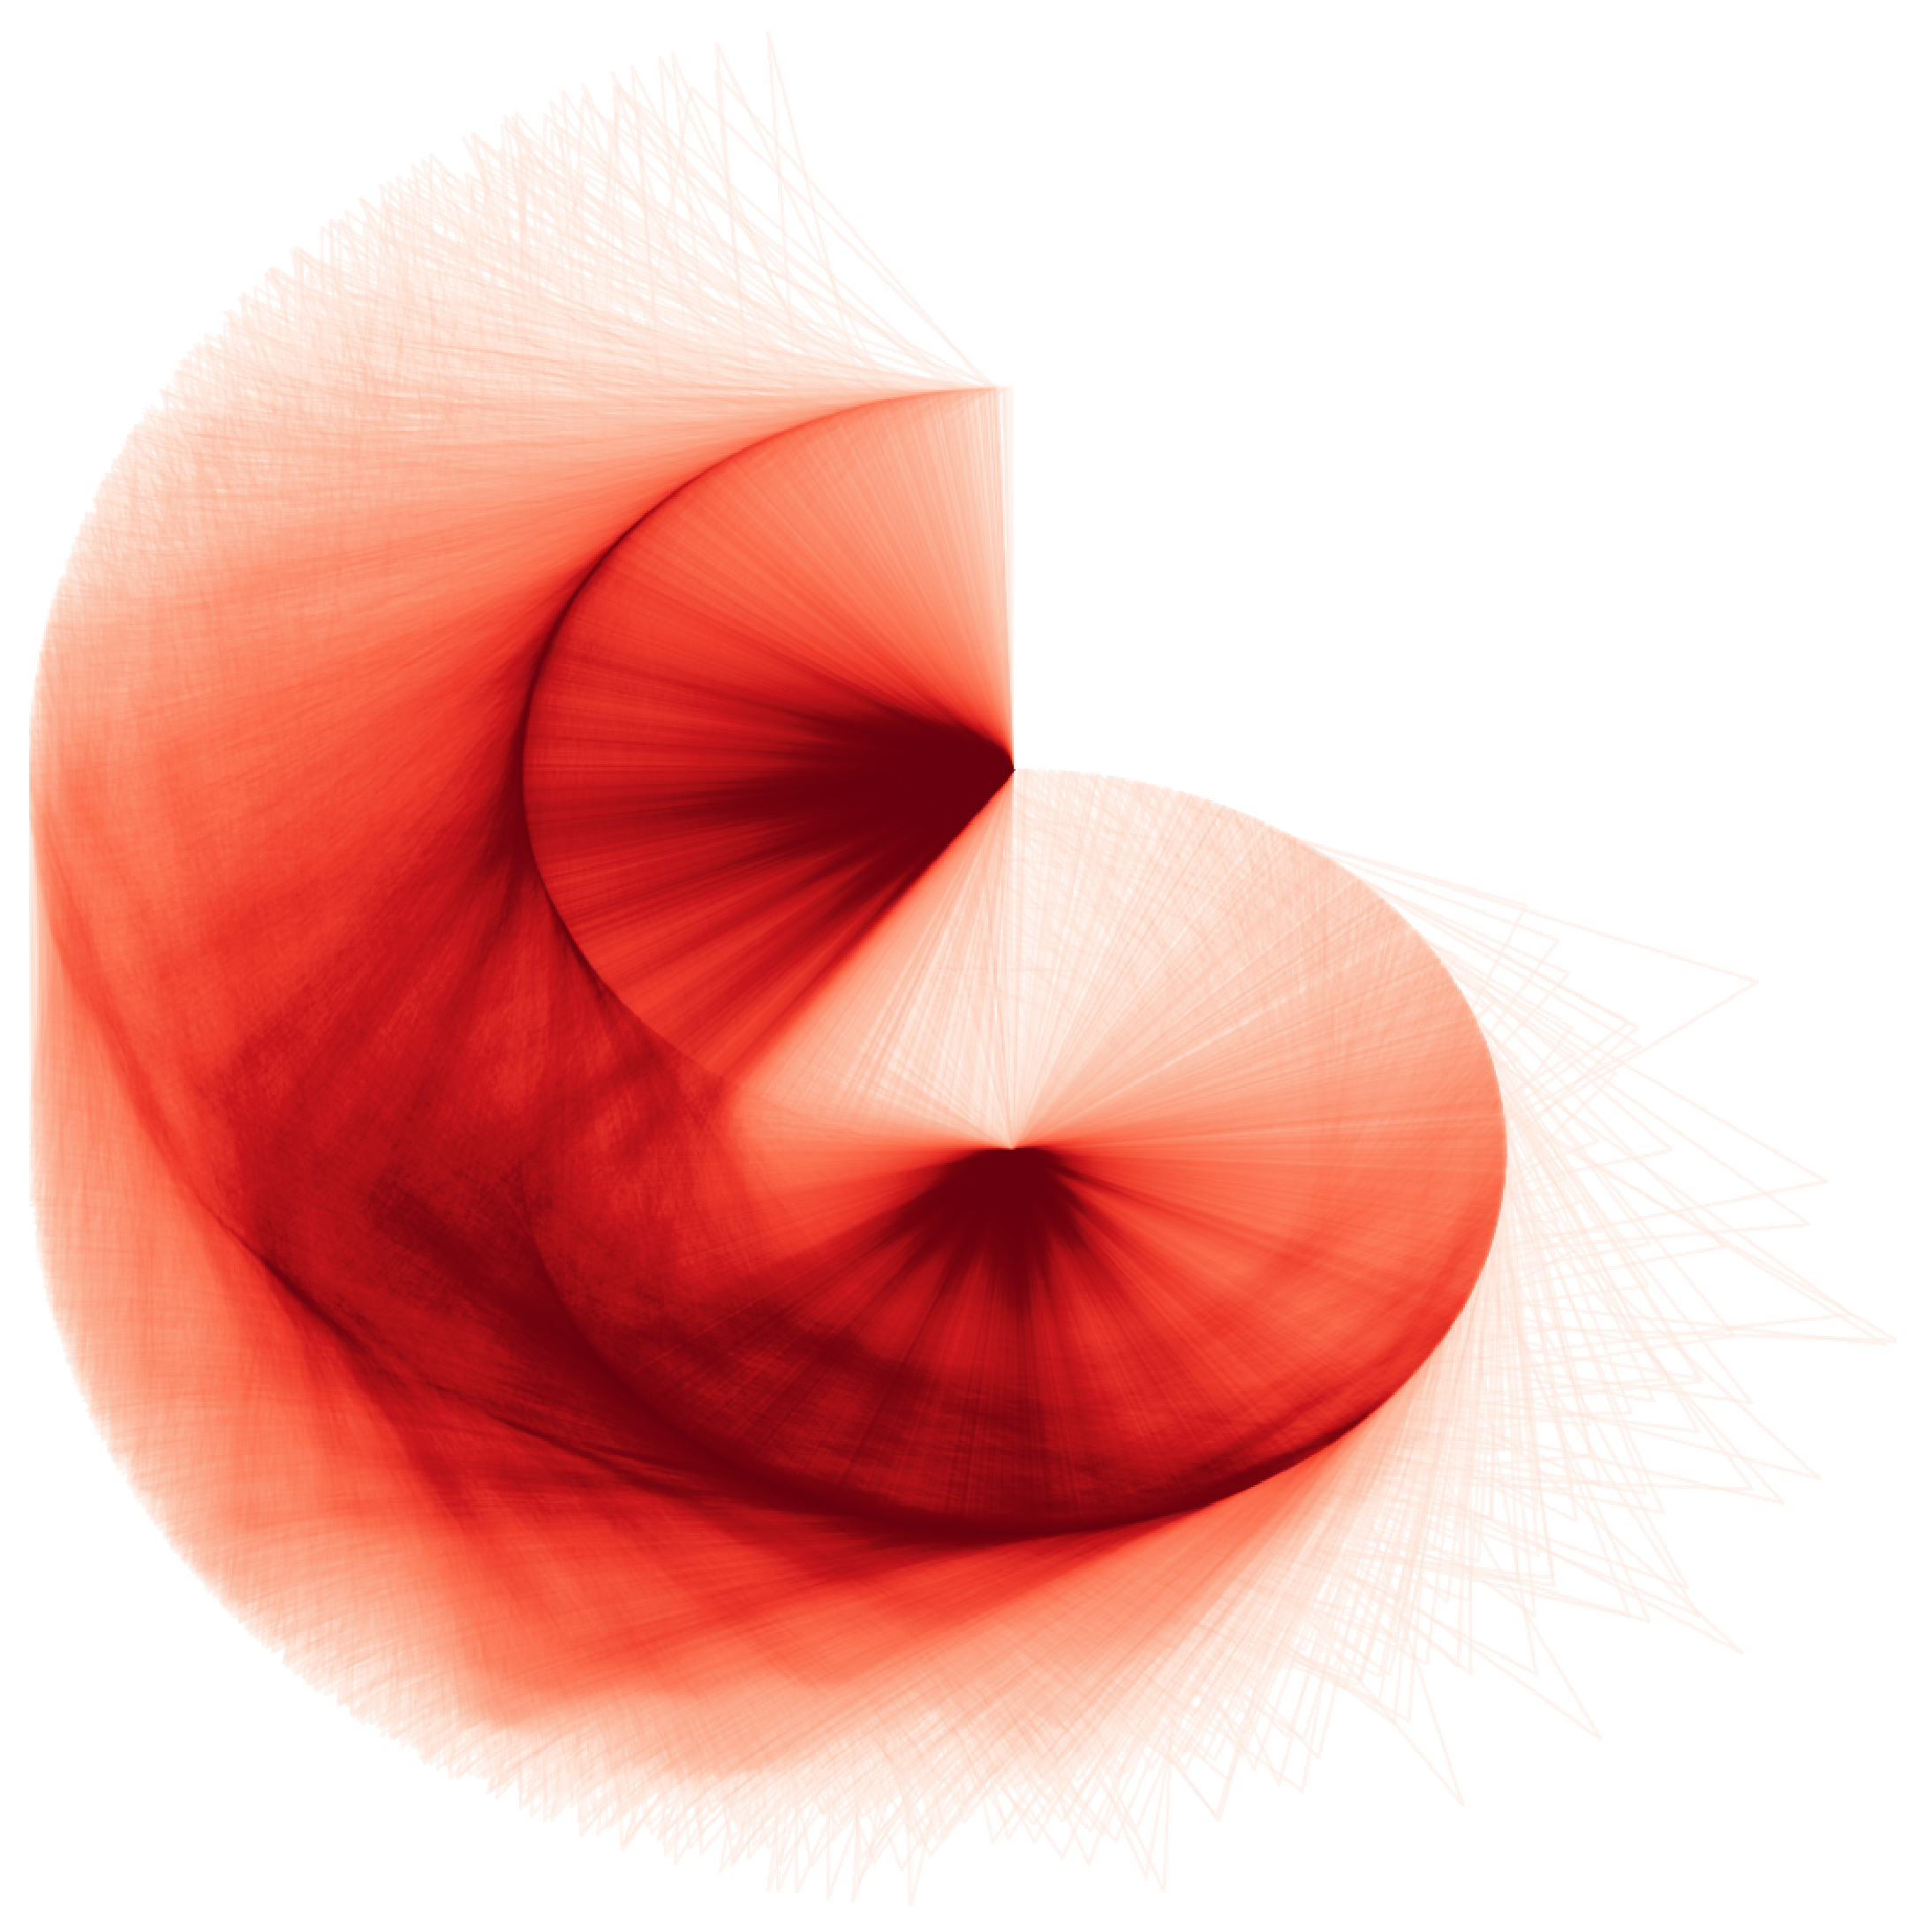
\includegraphics[width=\linewidth]{images/constraind_diffusion_rejection/loops_planar_rejection.pdf}
		\caption{Metropolis}
		\label{fig:loop_plot_sampled}
	\end{subfigure}
	\hfill
	\begin{subfigure}{0.19\textwidth}
		\centering
		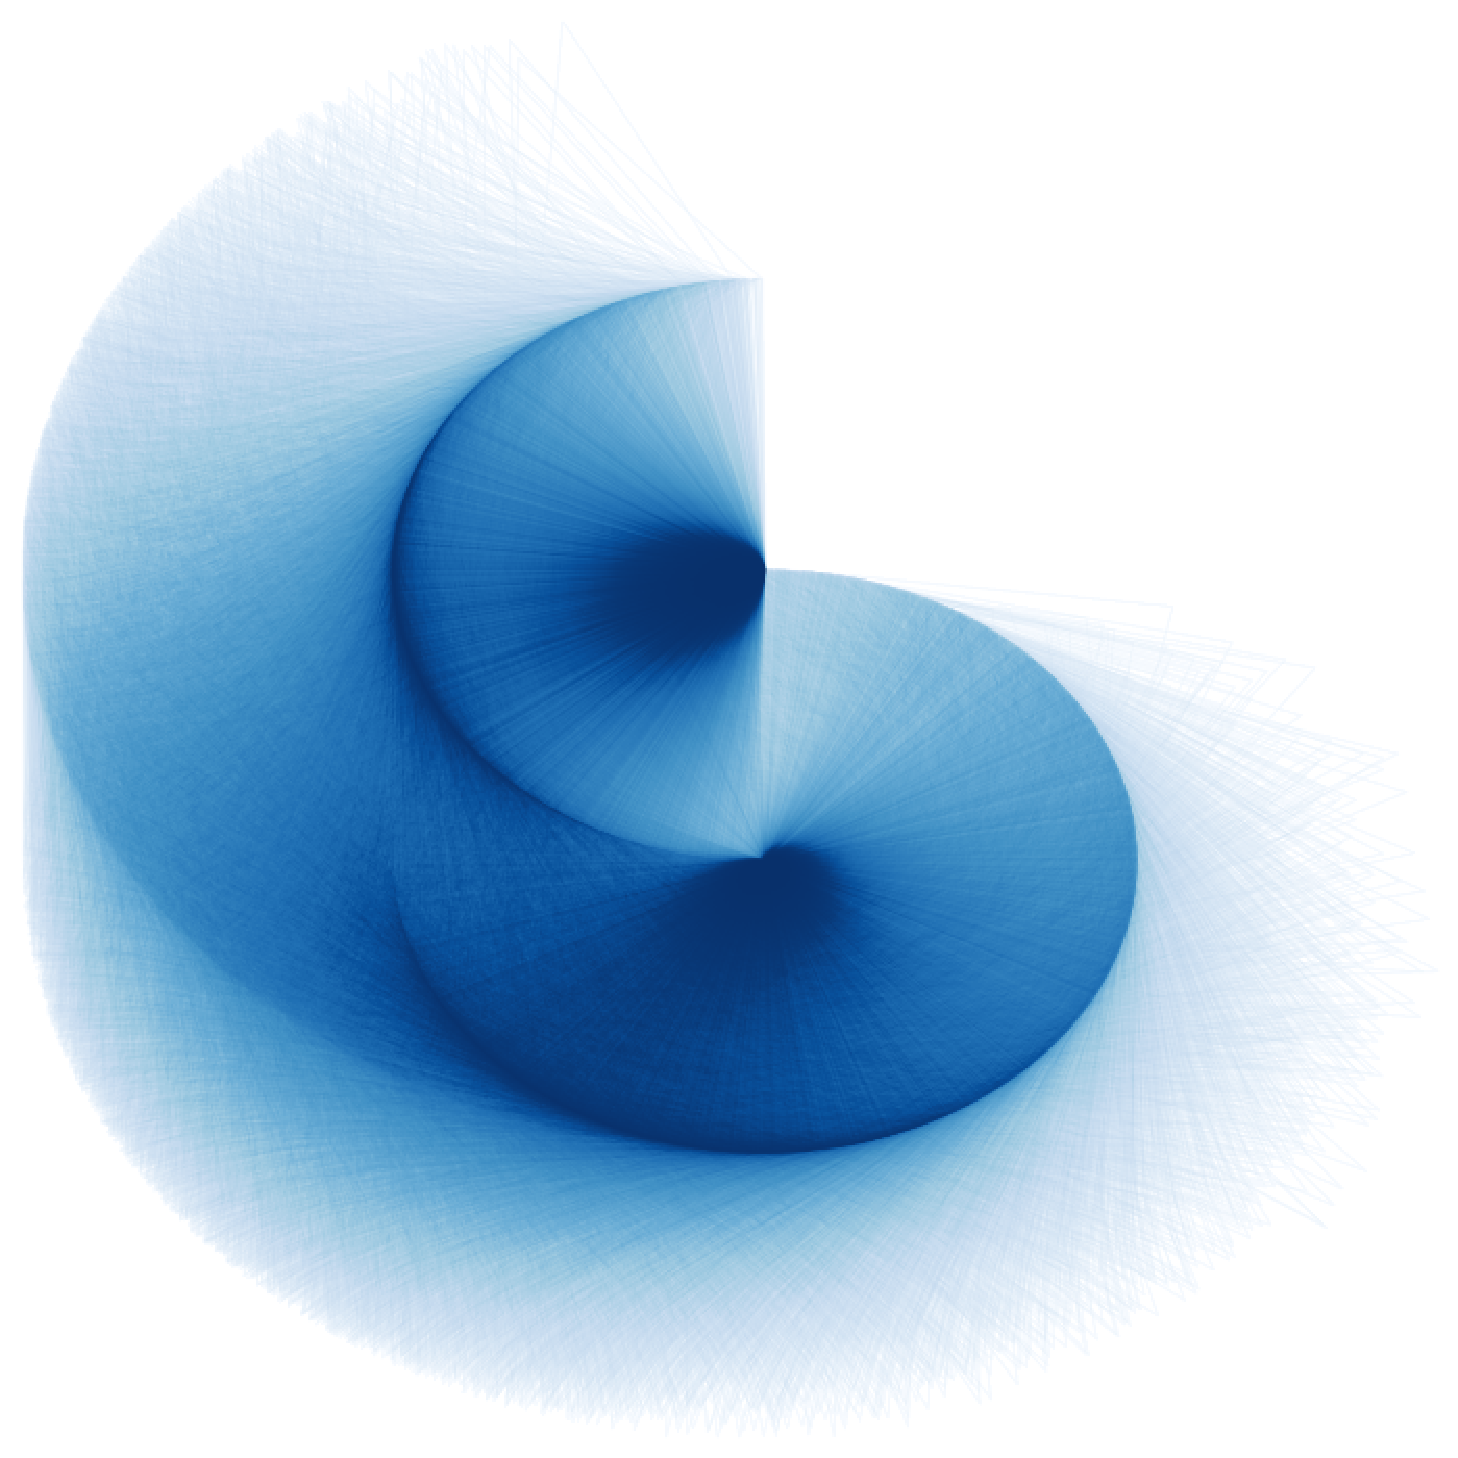
\includegraphics[width=\linewidth]{images/constrained_diffusion/loop_uniform_dist_2d.pdf}
		\caption{Uniform}
		\label{fig:loop_plot_uniform}
	\end{subfigure}
	\caption{Planar projection of the modelled \(C_\alpha\) chains from (a) the training dataset, (b-d) our models, and (e) the uniform distribution.
		Additional results and full correlation plots are postponed to~\Cref{sec:app_protein_exp}.
	}
	\label{fig:loop_plot}
\end{figure*}


To learn a distribution over this space, we leverage the methodology introduced in \cref{sec:constrained_diffusion_models} for the polytope component \(\mathbb{P}^3\) and in \cref{chp:riemannian_score_based_models} for the torus component \(\mathbb{T}^4\).
A qualitative comparison of samples from the data distribution, our log-barrier and reflected diffusion models, and the uniform distribution is presented in \Cref{fig:loop_plot}.
For enhanced visual clarity, we project the modelled spatial chain onto the 2D plane by removing the (unconstrained) torus component of the product manifold and only plotting the planar chains encoded by the (constrained) polytope component (a correlation plot of the full product manifold is presented in \Cref{fig:loops_pairs}).

It is immediately obvious that the data distribution is highly multimodal, encompassing a large number of locally optimal conformational clusters.
Nevertheless, both our reflected and log-barrier diffusion models are able to robustly approximate this challenging energetic landscape, producing samples that reflect key conformational states.
We present qualitative plots of the distributions in \cref{fig:loop_plot}.
For enhanced visual clarity, we project the modelled spatial chain onto the 2D plane by removing the (unconstrained) torus component of the product manifold and only plotting the planar chains encoded by the (constrained) polytope component.
A correlation plot of the full product manifold is presented in \todo{unify appendix plots}.

We present quantatiave MMD results in \cref{tab:loop_mmd_results}, which includes as a point of comparison the MMD between the uniform distribution and the data distribution.
The improved relative performance of the log-barrier method seems likely due to the fact that the data for this experiment is largely in the interior of the constrained set, not close to the boundary.


\begin{table}[h]
	\caption{
		Maximum mean discrepancy (MMD) (\(\downarrow\)) between samples from the trained model and a held-out test set from the robotics data.
		Means and standard deviations are computed over 3 different runs.
	}
	\label{tab:loop_mmd_results}
	\centering

	\begin{tabular}{rcccc}
		\toprule
		& {\scshape Log-Barrier}                & {\scshape Reflected}                  & {\scshape Metropolis} & {\scshape Uniform} \\
		\midrule
		\scshape MMD & \(0.032_{\pm{0.001}}\) & \(0.032_{\pm{0.021}}\) & \( 0.29_{\pm 0.03}\) & \(0.112_{\pm{0.001}}\) \\
		\bottomrule
	\end{tabular}
\end{table}

\subsection{Modelling geospatial data with non-convex country borders}
\label{sec:exp_constrained_country}

\subsection{Comparison with other methods for constrained diffusion models}
\begin{table*}
	\begin{tabular}{lccccc}
		                                             & \multicolumn{2}{c}{\(\overbracket{\mspace{200mu}}^{\text{Both required for fast DSM loss}}\)} &                                                                                                            \\%\multicolumn{2}{c}{\(\overbracket{\mspace{200mu}}^{\text{Preserves inductive biases}}\)} \\
		\toprule
		\scshape \bfseries Diffusion Model           & \scshape \thead{Tractable                                                                                                                                                                                  \\conditional score} & \scshape \thead{Simulation-free\\forward sampling} & \scshape \thead{Modelling                            \\domain}  & \scshape \thead{Preserves\\metric of \(\c{M}\)} \\
		\midrule
		Reflected Diffusions                                                                                                                                                                                                                                      \\
		\scshape \textcite{fishman2023diffusion_hl}  & \xmark                                                                                        & \xmark \hspace{0.1em} \(\del{\c{O}(?)}\) & Any \(\c{M}\)                                          & \cmark \\
		\scshape \textcite{fishman2023metropolis_hl} & \xmark                                                                                        & \xmark \hspace{0.1em} \(\del{\c{O}(?)}\) & Any \(\c{M}\)                                          & \cmark \\
		\scshape \textcite{lou2023reflected}         & \cmark                                                                                        & \cmark                                   & \(\sbr{0,1}^d \subset \R^d\)                           & \xmark \\

		\midrule
		Barrier Diffusions                                                                                                                                                                                                                                        \\
		\scshape \textcite{fishman2023diffusion_hl}  & \xmark                                                                                        & \xmark \hspace{0.1em} \(\del{\c{O}(?)}\) & \(\text{\small convex}\;{\subset}\;\text{any}\;\c{M}\) & \cmark \\
		\scshape \textcite{liu2023mirror}            & \cmark                                                                                        & \cmark                                   & \(\text{\small convex}\;{\subset}\;\R^d\)              & \xmark \\

		\bottomrule
	\end{tabular}
\end{table*}
